\documentclass[a4paper, 12pt]{scrartcl}
\usepackage[utf8]{inputenc}
\usepackage[english, ngerman]{babel}
\usepackage[T1]{fontenc}
\usepackage{amsmath}

%direkte pdf-links
\usepackage{hyperref}
%trassktript
\usepackage{xparse} 
\usepackage{enumitem}
\setlist[description]{
  font={\sffamily\bfseries},
  labelsep=0pt,
  labelwidth=\transcriptlen,
  leftmargin=\transcriptlen,
}
\newlength{\transcriptlen}
\NewDocumentCommand {\setspeaker} { mo } {%
  \IfNoValueTF{#2}
  {\expandafter\newcommand\csname#1\endcsname{\item[#1:]}}%
  {\expandafter\newcommand\csname#1\endcsname{\item[#2:]}}%
  \IfNoValueTF{#2}
  {\settowidth{\transcriptlen}{#1}}%
  {\settowidth{\transcriptlen}{#2}}%
}

%für Bilder
\usepackage{graphicx}
%deutsche anführungszeichen
\usepackage{csquotes}\MakeOuterQuote{"}
%ränder
\usepackage[left=3cm, right=4cm, top=3cm, bottom=2.5cm]{geometry}
\usepackage[numbers, round]{natbib}
%spacing
\usepackage[onehalfspacing]{setspace}
%Abkürzungsverzeichnis
\usepackage[printonlyused, footnote]{acronym}
%Anzeigen der restlichen Verzeichnisse
\usepackage{tocbibind}
%Literaturverzeichnis
\bibliographystyle{alphadin}
%größere Schriftgrößen als 17pt
\usepackage{lmodern}
%bessere umbrüche
\usepackage{microtype}
%Bildquellen
\newcommand*{\bildquelle}{%
  \footnotesize Quelle:
}
%römische zahlen
\newcommand{\RM}[1]{\MakeUppercase{\romannumeral #1{.}}}
\makeatletter
\newenvironment{folding}{\endgroup}{\begingroup \def \@currenvir{folding}\edef \@currenvline{\on@line}}
\makeatother

%für H-Bild-option
\usepackage{float}

\hyphenation{Schleu-sing-en Haupt-ein-kaufs-mö-glich-keit Nie-drig-preis-po-li-tik}

\title{Seminarfacharbeit}
\author{Toni Hausdörfer, Fabian Beez}
\date{27. Mai 2020}

\begin{document}
    \begin{titlepage}

    \raggedright
        Hennebergisches Gymnasium Georg Ernst\\
        Klosterstraße 2-4\\
        98554 Schleusingen
        
    \raggedleft\vspace*{-1.9cm}
        Jahrgang 2020/21
        
    
    \vfill\vfill\vfill\vfill\vfill\vfill

    \centering
        \LARGE\textbf{Seminararbeit}
        \vfill
        \large Onlinehandel und dessen Einfluss auf Kleinstädte und Dörfer im ländlichen Raum?\\[\baselineskip]\vfill
        
        von\\
        Toni Hausdörfer und Fabian Beez
    

    \vfill\vfill\vfill\vfill

    \raggedright
    Betreuende Lehrkraft:   Frau[?] Richter\\
    Abgabetermin:\\[\baselineskip]
    
\begin{tabular}[h]{|l|l|l|l|l|l|}
    \hline
    Bewertung & Note & Note in Worten & Punkte &  & Punkte \\
    \hline
    schriftliche Arbeit & & & & x 3 & \\
    \hline
    Präsentation & & & & x 1 & \\
    \hline
\end{tabular}

\vfill

\raggedleft
    Summe: \rule{1.5cm}{.4pt}\\
    Gesamtleistung nach \$ 61(7) GSO = Summe :2 (gerundet): \rule{1.5cm}{.4pt}\\[\baselineskip]\vfill\vfill\vfill
    \begin{tabular}{@{}l@{}}\hline
        Unterschrift des Kursleiters
    \end{tabular}
    
\vfill\vfill
\end{titlepage}

\newpage

    \input{exports/EidesstattlicheErklärung1.tex}
    \input{exports/EidesstattlicheErklärung.tex}
     
\vspace*{5cm}
\section*{Danksagung}
Zuerst möchten wir uns bei all denjenigen bedanken, die uns während der Anfertigung dieser Arbei unterstützt haben. 
Dazu zählen in erster Linie alle Teilnehmer der Umfragen.
Ein besonderer Dank gilt dabei Frau Karin Richter, die uns als betreuende Lehrkaft unterstützte.
\newpage


    \tableofcontents 
        \newpage

    \section{Einleitung}
        %?: mode beetz, ..., in schleusingen schließen immer mehr läden und es werden kaum neue eröffent(abgesehen von restoraunnts). gleichzeitig wird der onlineeinkauf immer attraktiver



Onlinehandel spielt eine immer größer werdende Rolle im Leben von Menschen fast aller Altersschichten. Aufgrund des allmählichen Verschwindens von Geschäften im Gebiet um Schleusingen haben wir uns die Frage gestellt, welche Rolle der Verkauf von Waren über das Internet in unserem Landkreis spielt, und ob die Schließungen einiger Geschäfte auf den Rückgang der Nachfrage für lokale Einzelhändler zurückzuführen ist.

Im Rahmen unserer Arbeit werden wir das Zutreffen folgender Thesen einschätzen:
\begin{itemize}
    \item Der Onlinehandel führt zu einem allmählichen Aussterben von stationären Händlern im ländlichen Bereich.
    
    \item Es gibt Waren, die nicht/kaum online gekauft werden.

    \item Der Onlinehandel schafft weniger Arbeitsplätze als indirekt verringert werden.
\end{itemize}

Außerdem werden wir auf Basis unserer Ergebnisse ein Konzept entwickeln, wie die Nachfrage und der Verkauf von Waren in unserem Landkreis erhöht werden kann.

        \newpage
    
    
    
    \section{Historie}
            %?: mode beetz, ..., in schleusingen schließen immer mehr läden und es werden kaum neue eröffent(abgesehen von restoraunnts). gleichzeitig wird der onlineeinkauf immer attraktiver



Onlinehandel spielt eine immer größer werdende Rolle im Leben von Menschen fast aller Altersschichten. Aufgrund des allmählichen Verschwindens von Geschäften im Gebiet um Schleusingen haben wir uns die Frage gestellt, welche Rolle der Verkauf von Waren über das Internet in unserem Landkreis spielt, und ob die Schließungen einiger Geschäfte auf den Rückgang der Nachfrage für lokale Einzelhändler zurückzuführen ist.

Im Rahmen unserer Arbeit werden wir das Zutreffen folgender Thesen einschätzen:
\begin{itemize}
    \item Der Onlinehandel führt zu einem allmählichen Aussterben von stationären Händlern im ländlichen Bereich.
    
    \item Es gibt Waren, die nicht/kaum online gekauft werden.

    \item Der Onlinehandel schafft weniger Arbeitsplätze als indirekt verringert werden.
\end{itemize}

Außerdem werden wir auf Basis unserer Ergebnisse ein Konzept entwickeln, wie die Nachfrage und der Verkauf von Waren in unserem Landkreis erhöht werden kann.

        \subsection{Entstehung und Entwicklung}
            PayPal fungiert in einer Onlinetransaktion als Zwischenhändler. Hierbei muss der Kunde aber bereits ein eingerichtetes und verlinktes Konto haben. Um sich bei PayPal zu registrieren muss man seinen Namen, seine E-Mail und eine Bankverbindung hinterlegen. Darauf wird einige Tage später ein kleiner Centbetrag überwiesen, zusammen mit einen Zahlencode, den man nur noch auf der Website eingeben muss, worauf das Konto freigeschaltet ist. Bei einer Kreditkarte ist es ein ähnliches Prozedere, wobei einige Cents abgebucht werden, bei beiden Methoden wird der Betrag ausgeglichen. Bei einem Kauf muss man vor dem Abschluss noch seine Daten seines Kontos, alias E-Mail und Passwort, was man nach eingeben des Zahlencodes einstellen kann, eintragen, diese werden dann von PayPal geprüft und der Kauf abgeschlossen. Dabei wird nicht einfach das Geld vom Konto des Käufers auf das Konto des Verkäufers gesendet. PayPal überweist das Geld direkt an das Konto des Händlers stellt aber erst Tage später per Lastschrift die Rechnung an den Käufer. Damit garantiert PayPal die schnellstmögliche Lieferung. Bei einer Rücksendung funktioniert PayPal ähnlich. Dabei wird das Geld direkt auf den PayPal-Konto gutgeschrieben, darauf ist es möglich sich auch das Geld auf sein Bankkonto überweisen zu lassen \cite{schulz}. Auch ist es möglich Geld zu transferieren, wenn es um keinen Kauf bzw. keinen Kauf auf einer Internetseite mit PayPal geht. Durch die PayPal App wurde auch das Senden vereinfacht speziell an Nahestehende, wie Freunde und Familie. Auch hat PayPal eine Funktion namens Moneypool. Hierbei handelt es sich um eine Art extra Konto, dass für einen einzigen Zweck eingerichtet worden ist. Darauf können ausgesuchte Personen, vom Ersteller voreingestellt, zugriff haben, dabei können sie aber nur Geld zum „Pool“ hinzufügen, daher auch der Name. Dadurch können beispielsweise Geschenke oder Überraschungen finanziert werden, egal ob es sich um Familienmitglieder handelt oder Arbeitskollegen, solange jeder als Freund registriert ist vom Ersteller des Moneypools \cite{PayPal}. PayPals Ziel war es Bezahlen online sicherer zu machen. Dabei stehen drei Punkte im Vordergrund: Käuferschutz, Datensicherheit, Transaktionssicherheit. Beim Käuferschutz handelt es sich um eine Regelung wobei, wenn die Beschreibung eines Artikels inakkurat ist oder der Artikel gar nicht erst ankommt, dann die volle Summe samt Porto-Gebühren auf das Konto des Käufers zurücküberwiesen wird. Die Datensicherheit ist der Vorteil, dass man seine Bankdaten nicht mit dem ganzen Internet teilen muss, sondern nur mit PayPal die alle kommenden Geschäfte für einen Abwickeln. Ebenfalls ist jede Transaktion und E-Mail von PayPal verschlüsselt wodurch die Transaktionen so sicher wie möglich versucht gestaltet zu werden. All dies hat seine Kosten, zumindest für Händler. Jegliche Transaktion von Privatpersonen sind kostenlos, solang sie im selben Land registriert sind und keine Währungsumrechnung notwendig ist. Hingegen gelten für Händler Raten, worin sie nach höheren Transaktionsvolumen höhere Gebühren zahlen müssen.

\begin{figure}[h]
    \begin{center}
        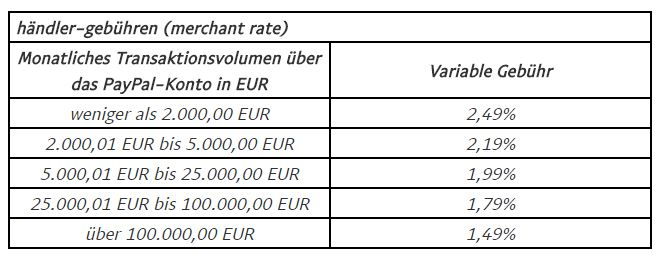
\includegraphics[width=8cm]{media/paypal.png}
        \caption{Paypal's Gebühren}
        \label{gebühren-paypal}
        \bildquelle Paypal erhöht Gebühren für Händler. In: Sellercamp (2019). https://bit.ly/3nWdMna. – aufgerufen am 22. 12. 2020
    \end{center}
\end{figure}

\noindent PayPal versucht eine Alternative zu herkömmlichen Bezahlungsmethoden zu sein, obwohl die Sicherheit und der Service von PayPal auch von anderen Unternehmen geleistet werden kann.

        \subsection{Zusammenhang zwischen Onlinemarketing und -handel}
            <<<<<<< Updated upstream
Auch wenn PayPal seine Vorteile mit sich bringt hat es seine Nachteile. Speziell die weitere Nutzung der Daten, die PayPal generiert, ist fraglich. Dabei sendet PayPal Daten an das US-Heimatschutzministerium die die Daten abgleicht mit möglichen Straftätern oder Terroristen, dabei kann schon der geringste Verdacht zu einer Sperrung des Kontos führen. (https://www.it-recht-kanzlei.de/Brauchen_wir_PayPal.html) Ebenfalls ist das Einfrieren von Konten auch ein großer Nachteil, da eine Vielzahl von Menschen der Geldwäsche von PayPal bezichtigt werden, aber ohne jeglichen Beweis. In beiden Fällen kann man Wiederspruch einlegen, aber man muss Nachweißen das alle Zahlungen legal waren und sich ausweisen können. Bis zu dem Zeitpunkt der Wiedereröffnung des Kontos oder Wiederaktivierung falls der Wiederspruch angenommen worden ist können einige Monate vergehen und man hat absolut keinen Zugriff auf das Geld. Dazu hat man keinen Ansprechpartner in Deutschland für einen Beschwerde, sondern muss sich an die englische Behörde wenden, wodurch auch englisches Recht gilt, dadurch ist das Unternehmen nahezu unantastbar in Deutschland. 
=======




Durch diese Grundstrukturen hat sich ein Wirtschaftssektor gebildet der profitabelste Sektor für ein großes Unternehmen ist. Besonders durch die Einbeziehung des Onlinehandels konnte der E-Commerce erst seinen Aufstieg feiern. Jedoch ist das Potential des Sektors noch lange nicht ausgeschöpft. Durch die Entwicklung von Sprachassistenten und Künstlichen Intelligenzen wird die Zeit des Prozesses des Einkaufens bis zum minimalen verringert. Auch durch das Integrieren von Drohen wird die Allgegenwärtigkeit des Onlinehandels früher oder später offensichtlich. %(https://www.tagesschau.de/wirtschaft/amazon-drohnen-101.html) 
Die Steigerung des Kommerzes, ins besonderen in ländlichen Regionen ist überwältigend. Vom Jahr 2000 bis 2020 hat sich der Umsatz in Deutschland mehr als verfünfzigfacht. Von 1,3 Milliarden € auf 59,2 Milliarden € in nur zwanzig Jahren. %(https://de.statista.com/statistik/daten/studie/3979/umfrage/e-commerce-umsatz-in-deutschland-seit-1999/)
Auch zeigen die tendenzen in den kommenden Jahren nur nach oben. Bis 2023 sollen 71,4 Milliarden € Umsatz im Sektor E-Commerce gemacht werden.       
 
%(https://parcellab.com/wp-content/uploads/2019/09/statistic_id488012_prognose-der-e-commerce-nutzer-in-deutschland-bis-2023.png) 
>>>>>>> Stashed changes

        \newpage
        
        
        
    \section{PayPal}
		%?: mode beetz, ..., in schleusingen schließen immer mehr läden und es werden kaum neue eröffent(abgesehen von restoraunnts). gleichzeitig wird der onlineeinkauf immer attraktiver



Onlinehandel spielt eine immer größer werdende Rolle im Leben von Menschen fast aller Altersschichten. Aufgrund des allmählichen Verschwindens von Geschäften im Gebiet um Schleusingen haben wir uns die Frage gestellt, welche Rolle der Verkauf von Waren über das Internet in unserem Landkreis spielt, und ob die Schließungen einiger Geschäfte auf den Rückgang der Nachfrage für lokale Einzelhändler zurückzuführen ist.

Im Rahmen unserer Arbeit werden wir das Zutreffen folgender Thesen einschätzen:
\begin{itemize}
    \item Der Onlinehandel führt zu einem allmählichen Aussterben von stationären Händlern im ländlichen Bereich.
    
    \item Es gibt Waren, die nicht/kaum online gekauft werden.

    \item Der Onlinehandel schafft weniger Arbeitsplätze als indirekt verringert werden.
\end{itemize}

Außerdem werden wir auf Basis unserer Ergebnisse ein Konzept entwickeln, wie die Nachfrage und der Verkauf von Waren in unserem Landkreis erhöht werden kann.

        \subsection{Entstehung und grobe Funktionsweise}
            PayPal fungiert in einer Onlinetransaktion als Zwischenhändler. Hierbei muss der Kunde aber bereits ein eingerichtetes und verlinktes Konto haben. Um sich bei PayPal zu registrieren muss man seinen Namen, seine E-Mail und eine Bankverbindung hinterlegen. Darauf wird einige Tage später ein kleiner Centbetrag überwiesen, zusammen mit einen Zahlencode, den man nur noch auf der Website eingeben muss, worauf das Konto freigeschaltet ist. Bei einer Kreditkarte ist es ein ähnliches Prozedere, wobei einige Cents abgebucht werden, bei beiden Methoden wird der Betrag ausgeglichen. Bei einem Kauf muss man vor dem Abschluss noch seine Daten seines Kontos, alias E-Mail und Passwort, was man nach eingeben des Zahlencodes einstellen kann, eintragen, diese werden dann von PayPal geprüft und der Kauf abgeschlossen. Dabei wird nicht einfach das Geld vom Konto des Käufers auf das Konto des Verkäufers gesendet. PayPal überweist das Geld direkt an das Konto des Händlers stellt aber erst Tage später per Lastschrift die Rechnung an den Käufer. Damit garantiert PayPal die schnellstmögliche Lieferung. Bei einer Rücksendung funktioniert PayPal ähnlich. Dabei wird das Geld direkt auf den PayPal-Konto gutgeschrieben, darauf ist es möglich sich auch das Geld auf sein Bankkonto überweisen zu lassen \cite{schulz}. Auch ist es möglich Geld zu transferieren, wenn es um keinen Kauf bzw. keinen Kauf auf einer Internetseite mit PayPal geht. Durch die PayPal App wurde auch das Senden vereinfacht speziell an Nahestehende, wie Freunde und Familie. Auch hat PayPal eine Funktion namens Moneypool. Hierbei handelt es sich um eine Art extra Konto, dass für einen einzigen Zweck eingerichtet worden ist. Darauf können ausgesuchte Personen, vom Ersteller voreingestellt, zugriff haben, dabei können sie aber nur Geld zum „Pool“ hinzufügen, daher auch der Name. Dadurch können beispielsweise Geschenke oder Überraschungen finanziert werden, egal ob es sich um Familienmitglieder handelt oder Arbeitskollegen, solange jeder als Freund registriert ist vom Ersteller des Moneypools \cite{PayPal}. PayPals Ziel war es Bezahlen online sicherer zu machen. Dabei stehen drei Punkte im Vordergrund: Käuferschutz, Datensicherheit, Transaktionssicherheit. Beim Käuferschutz handelt es sich um eine Regelung wobei, wenn die Beschreibung eines Artikels inakkurat ist oder der Artikel gar nicht erst ankommt, dann die volle Summe samt Porto-Gebühren auf das Konto des Käufers zurücküberwiesen wird. Die Datensicherheit ist der Vorteil, dass man seine Bankdaten nicht mit dem ganzen Internet teilen muss, sondern nur mit PayPal die alle kommenden Geschäfte für einen Abwickeln. Ebenfalls ist jede Transaktion und E-Mail von PayPal verschlüsselt wodurch die Transaktionen so sicher wie möglich versucht gestaltet zu werden. All dies hat seine Kosten, zumindest für Händler. Jegliche Transaktion von Privatpersonen sind kostenlos, solang sie im selben Land registriert sind und keine Währungsumrechnung notwendig ist. Hingegen gelten für Händler Raten, worin sie nach höheren Transaktionsvolumen höhere Gebühren zahlen müssen.

\begin{figure}[h]
    \begin{center}
        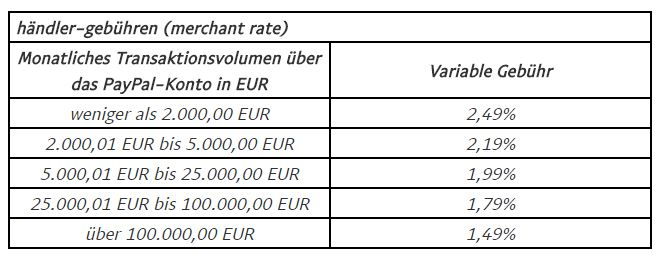
\includegraphics[width=8cm]{media/paypal.png}
        \caption{Paypal's Gebühren}
        \label{gebühren-paypal}
        \bildquelle Paypal erhöht Gebühren für Händler. In: Sellercamp (2019). https://bit.ly/3nWdMna. – aufgerufen am 22. 12. 2020
    \end{center}
\end{figure}

\noindent PayPal versucht eine Alternative zu herkömmlichen Bezahlungsmethoden zu sein, obwohl die Sicherheit und der Service von PayPal auch von anderen Unternehmen geleistet werden kann.

        \subsection{Negative Folgen}
            <<<<<<< Updated upstream
Auch wenn PayPal seine Vorteile mit sich bringt hat es seine Nachteile. Speziell die weitere Nutzung der Daten, die PayPal generiert, ist fraglich. Dabei sendet PayPal Daten an das US-Heimatschutzministerium die die Daten abgleicht mit möglichen Straftätern oder Terroristen, dabei kann schon der geringste Verdacht zu einer Sperrung des Kontos führen. (https://www.it-recht-kanzlei.de/Brauchen_wir_PayPal.html) Ebenfalls ist das Einfrieren von Konten auch ein großer Nachteil, da eine Vielzahl von Menschen der Geldwäsche von PayPal bezichtigt werden, aber ohne jeglichen Beweis. In beiden Fällen kann man Wiederspruch einlegen, aber man muss Nachweißen das alle Zahlungen legal waren und sich ausweisen können. Bis zu dem Zeitpunkt der Wiedereröffnung des Kontos oder Wiederaktivierung falls der Wiederspruch angenommen worden ist können einige Monate vergehen und man hat absolut keinen Zugriff auf das Geld. Dazu hat man keinen Ansprechpartner in Deutschland für einen Beschwerde, sondern muss sich an die englische Behörde wenden, wodurch auch englisches Recht gilt, dadurch ist das Unternehmen nahezu unantastbar in Deutschland. 
=======




Durch diese Grundstrukturen hat sich ein Wirtschaftssektor gebildet der profitabelste Sektor für ein großes Unternehmen ist. Besonders durch die Einbeziehung des Onlinehandels konnte der E-Commerce erst seinen Aufstieg feiern. Jedoch ist das Potential des Sektors noch lange nicht ausgeschöpft. Durch die Entwicklung von Sprachassistenten und Künstlichen Intelligenzen wird die Zeit des Prozesses des Einkaufens bis zum minimalen verringert. Auch durch das Integrieren von Drohen wird die Allgegenwärtigkeit des Onlinehandels früher oder später offensichtlich. %(https://www.tagesschau.de/wirtschaft/amazon-drohnen-101.html) 
Die Steigerung des Kommerzes, ins besonderen in ländlichen Regionen ist überwältigend. Vom Jahr 2000 bis 2020 hat sich der Umsatz in Deutschland mehr als verfünfzigfacht. Von 1,3 Milliarden € auf 59,2 Milliarden € in nur zwanzig Jahren. %(https://de.statista.com/statistik/daten/studie/3979/umfrage/e-commerce-umsatz-in-deutschland-seit-1999/)
Auch zeigen die tendenzen in den kommenden Jahren nur nach oben. Bis 2023 sollen 71,4 Milliarden € Umsatz im Sektor E-Commerce gemacht werden.       
 
%(https://parcellab.com/wp-content/uploads/2019/09/statistic_id488012_prognose-der-e-commerce-nutzer-in-deutschland-bis-2023.png) 
>>>>>>> Stashed changes

        \newpage
        
        
        
    \section{Konsumverhalten}
             Amazon ist ein Onlineversandhändler, der eine breite Bekanntheit genießt und vor allem im europäischen Raum im Bereich des Onlinehandels einen großen Anteil ausmacht. Während Aliexpress in Asien und östlichen Teilen Europas und Ebay im Norden der EU stark vertreten sind, ist Amazon in Zentral-, Nord- und Westeuropa die Plattform mit dem größten Wert von Verkäufen\cite[S. 22]{EuroCommerce}. Außerdem macht Amazon bereits seit Ende 2017 mehr als die Hälfte der Verkäufe durch Drittanbieter aus\cite[S. 25]{Haendlerbund}. Dementsprechend werde ich in den folgenden Unterpunkten die Firma in Bezug auf ihre Entwicklung, die Auswirkungen dieser und der Konkurrenzfähigkeit zu lokalen Händlern analysieren und auf Basis der Erkentnisse Schlussfolgerungen im Bezug auf Schleusingen und des hildburghäuser Landkreis schließen.

        \subsection{Konsumverhalten und dessen Veränderung bezüglich der Vertriebsstrukturen}
            \iffalse
Einteilung in: Online-Marktplätze + Online-Händler, Intermediäre, Kataloversender, stationäre Händler, Hersteller/Marken \cite{Graf}

entwicklung des kaufprozesses: graf:abbildung; 

https://edoc.sub.uni-hamburg.de/hcu/volltexte/2017/370/pdf/Ebert_Kirsten.pdf Anfang

änderung kaufablauf: \cite{Schaefers}
\fi

% ALLGEMEIN
Bis Anfang 2020 war das Konsumverhaten in Deutschland im Allgemeinen geprägt durch eine starkte Kaufkraft, z. T. dank dem 0\%-igen Leitzins der \ac{EZB}\cite[S. 49]{Ebert} - jedoch ist die Kaufkraft durch die derzeit vorherrschende Corona-Situation abgeschwächt worden\cite{BfWE}. 

Außerdem haben sich die Bedürfnisse innerhab der letzten Jahrzente stark geändert: statt gleichbleibenden, rationalen Käufen und Kaufmotiven in den 1950ern, die die Auswahl der gekauften Güter stark abhängig von der zur Verfügung stehenden Geldmenge machten\cite[S. 38]{Schramm}; herrscht heute ein deutlich dynamischeres Kaufklima:
\begin{quote}
"So beziehen jetzt zum Beispiel auch solvente Kunden ihre Lebensmittel aus dem Billigdiscounter, während  umgekehrt  einkommensschwächere  Schichten  zu  Luxusgütern  greifen."\cite[S. 43]{Nitt}
\end{quote}

Im folgendem werde ich Verkäufer aller Art ähnlich wie im Buch "Das E-Commerce Buch: Marktanalysen - Geschäftsmodelle - Strategien" unterteilen: in Online-Marktplätze, Online-Händler, Kataloversender, stationäre Händler und Hersteller\cite[S. 18ff]{Graf}. Dabei sind Online-Marktplätze eine Art Online-Vermittler zwischen Kunden und Verkäfer, Online-Händler bieten dagegen nur eigene, meist sehr spezialisierten Sortimente an. Kataloversender verhalten sich ähnlich: sie versenden ihr Sortiment direkt an Kunden. Stationäre Händler verkaufen im Gegensatz zu den genannten Verkaufstrukturen in Fillialen und sind am stärksten von den Änderungen der letzten Jahrzenten betroffen. Während sich die genannten Unternehmensarten meistens am Ende der Verkaufskette befinden, stehen Händler oft am Anfang: sie stellen Güter her und sind dementsprechend, insofern sie nicht selber verkaufen, auf weitere Unternehmen für Verkauf und Vermarktung angewiesen(ebd.). %vor und -nachteile?, beispielsunternehmen


\iffalse 
    VERÄDERUNGEN bzgl der Verkäuferstruktur
    
        individiuelle Produkte
        
        sozialer Aspekt: Einzelhandel
        
        Einzelhandel: erst anbieter, dann produkt; onlinehandel umgekehrt
            .> weil einfacheres vergleichen, mehrere läden lohnen sich nicht
            einzelhandel weniger preissensibel; jedoch ist onlinehandel vor allem in der Elektronikbranche konkurrenzfähig, sh. Media Markt\cite[S. 27]{Graf}
            ABBILDUNG GABLER S. 313
        Mutichannel: Onlinebestellung im laden abholen/zurückgeben, wenig mehrwert (S 37) 
            
        {
        Katalogversender bieten ab 2002 online an: +56\% Umsatz, S. 30f
        }
        
        Hersteller: "Powerseller" kaufen produkte von herstellern, verkaufen siedeutlich unter marktpreisen weiter -> probleme mit preisverfall S. 31
        schrecken aufgrund von biosherigen vertreib über fachhandel meist davor zurück, online-marktplätze einzurichten, vereinzelt(hugoboss.com) S. 34
        
        allgemein online: großes wachstum ab 2002 S. 32
            jüngere kaufen mehr online ein S 37f
            
    STEHENGEBLIEBEN: S 39
\fi

Zusätzlich hat sich unter vielen Konsumenten das Bedürfnis nach individiuellen und auf den Käufer angepassten Produkten gebildet\cite[S. 43]{Nitt}, was wahrscheinlich durch die extrem große Außwahl bei dem Online-Shopping hervorgerufen wurde. In diesem Aspekt kann der stationäre Einzelhandel schlicht nicht mithalten, da Raum für Produkte begrenzt und sehr teuer ist. 
\iffalse
> billig - strategie vorallem von amazon und alibaba

veranschaulichung eigene tabelle börsenwert einzelner unternehmen

Dabei gibt es auch unternehmen, die mehrere berieche nutzen, wie amazon
\fi

Allerdings hat der stationäre Handel noch einen bedeutenden Vorteil: den sozialen Aspekt. Dieser wird vermutlich mit fortschreitender Digitalisierung eine immer wichtigere Rolle spielen\cite[S. 50]{Ebert}.
\begin{quote}
"Als Mittel gegen Vereinsamung und Anonymisierung im Alltag wird die soziale Komponente beim Einkaufen [...] zunehmend an Bedeutung gewinnen."\cite[S. 43]{Nitt}
\end{quote}

            
        \subsection{Einschätzung und Folgen}
            %zusammenfassung

%gegenseitige beeinflussung: showrooming-effekt: kauf online aufgrund von stationärere beratung -- kauf stationär nach onlinerecherche \cite[S. 21f]{evilcom}

%wie viele läden haben in schleusingen einen onlineshop?


\begin{folding} %stationärer Handel

Aufgrund der Verschiebung von Nachfrage und Bedürfnissen von Konsumenten in den letzten Jahrzehnten wird der stationäre Handel trotz Multichannel-Versuchen keine einfache Zukunft haben. So kann in vielen Fällen stattdessen direkt von Herstellern gekauft werden, die mittlerweile den Vertriebswegwechsel von \ac{B2B} zu \ac{B2C} weitesgehend hinter sich haben. 
Insbesondere in Thüringen steht es im Vergelich zum Rest Deutschlands dank der Kombination aus schlechter Kaufkraft und niedriger Bevölkerungszahl pro Fläche schlecht um den konventionellen Einzelhandel\cite[S. 29]{Nitt}. Dazu kommen demografische Änderungen, die insbesondere in der Mitte Deutschlands Probleme verursachen: so nimmt die Bevölkerung z. B. in Hamburg, trotz Schrumpfen der Bevölkerungszahl, zu - jedoch nicht in Hildburghausen, einer der Landkreise, die am meisten Bewohner verliert\cite[S. 32f]{Nitt}. 
Zum Glück einiger Vertriebe treffen diese schlechten Chancen nicht auf alle Branchen zu - der Lebensmittelvertrieb hat z. B. kaum Online-Konkurrenz[Umfrage]. Um in den restlichen Geschäftssektoren einen maximale großen Umsatz zu erzielen, sollte der konventionelle Einzelhandel aufgrund der alternden Bevölkerung, die meist noch stationär kauft, vorerst Investitionen für die wachsende Gruppe von Senioren und dementsprechend Erreichbarkeit o. ä. nutzen.

\end{folding}

\begin{folding} %Umweltverschmutzung

Zudem kommt immer öfter das Argument auf, dass der Wechsel zum Onlinehandel umweltschädlich sei, da mehr Lieferfahrzeuge unterwegs sind. Jedoch haben bereits die Autoren des "Evil Commerce [...]"-Buches diese These anhand einer Modellrechnung weitesgehend wiederlegt. Sie berechneten eine 90\%-ige Kraftstoffersparniss bei komplettem Umstieg zum Distanzhandel in Großstädten unter optimalen Bedingungen\cite[S. 25f]{evilcom}. Um genauerer Aussagen bezüglich des ländlichen Raumes zu treffen, werde ich die genannte Rechnung bzgl. Entfernung - da Einkaufszentren nicht berücksichtigt wurden - modifizieren und insofern erweitern, dass zusätzlich ein Einkauf in mehreren Geschäften nacheinander mit in Betracht gezogen wird.

\begin{itemize}

\item Im meiner Modellrechnung kaufen 100 Bewohner eines Dorfes in einer 4km entfernten Stadt ein. Sie kaufen im Durchschnitt in 3 von 10 Einkaufsmöglichkeiten ein, die je 500m voneinander entfernt sind. Dabei gehe ich davon aus, dass alle Kunden über eine 500m lange Straße innerhalb des Dorfes zu erreichen sind.

\item Wenn alle Bewohner stationär kaufen, legen sie im Durchschnitt eine Strecke von 

\begin{align}(250m + 4000m + 3 \cdot 500m + 4000m + 250m) \cdot 100 = 1000000m\end{align}

 zurück. Dabei nehme ich an, dass alle Bewohner denselben Ortsausgang benutzen und somit einen durchschnittlichen Weg von 250m zu diesem besitzen.

\item Wenn jeder Verkäufer jedoch die Güter an seine im Durchschnitt 30 Kunden versendet, müssten alle Lieferwagen zusammen eine Strecke von gerade einmal 

\begin{align}(4000m + 500m + 4000m) \cdot 10 = 85000m\end{align}

zurücklegen.
\item In dieser Darstellung hat der Distanzhandel eine ähnlich hohe Kraftstoffersparniss - 91.5\%. 

\end{itemize}
Zwar kann mithilfe dieses Modelles die These der Umweltverschmutzung auch auf dem Land im Allgemeinen wiederlegt werden, jedoch ist sie keine genaue Darstsellung der Realität, da viele Faktoren, wie z. B. die Retouranzahl, die beispielsweise in der Modebranche überproportional hoch ist, nicht beachtet wurden(ebd.).

\end{folding}

        \newpage
            
            
            
    \section{Wirtschaft mit Blick auf Unternehmen}
            Der Onlinehandel hat den Verkauf, speziell von kleineren Märkten, revolutioniert. Nicht nur durch Onlinemarketing, sondern auch durch den Verkauf auf Seiten anderer Anbieter konnten Unternehmen ihre Kundenzahl erhöhen und ihre Profite maximieren. Auch Produkte, die durch Handarbeit hergestellt werden, konnten ihre Position im Markt finden und sich meist als Luxusgut etablieren. Ebenfalls konnten sicherlich auch, durch das schlechte Marketing kleiner Betriebe online, Unternehmen wie Amazon oder Ebay das Loch im Markt nutzen um zu den Multi-Milliarden-Konzernen zu werden die sie heute sind.      

        \subsection{Entwicklung der Wirtschaft}
            PayPal fungiert in einer Onlinetransaktion als Zwischenhändler. Hierbei muss der Kunde aber bereits ein eingerichtetes und verlinktes Konto haben. Um sich bei PayPal zu registrieren muss man seinen Namen, seine E-Mail und eine Bankverbindung hinterlegen. Darauf wird einige Tage später ein kleiner Centbetrag überwiesen, zusammen mit einen Zahlencode, den man nur noch auf der Website eingeben muss, worauf das Konto freigeschaltet ist. Bei einer Kreditkarte ist es ein ähnliches Prozedere, wobei einige Cents abgebucht werden, bei beiden Methoden wird der Betrag ausgeglichen. Bei einem Kauf muss man vor dem Abschluss noch seine Daten seines Kontos, alias E-Mail und Passwort, was man nach eingeben des Zahlencodes einstellen kann, eintragen, diese werden dann von PayPal geprüft und der Kauf abgeschlossen. Dabei wird nicht einfach das Geld vom Konto des Käufers auf das Konto des Verkäufers gesendet. PayPal überweist das Geld direkt an das Konto des Händlers stellt aber erst Tage später per Lastschrift die Rechnung an den Käufer. Damit garantiert PayPal die schnellstmögliche Lieferung. Bei einer Rücksendung funktioniert PayPal ähnlich. Dabei wird das Geld direkt auf den PayPal-Konto gutgeschrieben, darauf ist es möglich sich auch das Geld auf sein Bankkonto überweisen zu lassen \cite{schulz}. Auch ist es möglich Geld zu transferieren, wenn es um keinen Kauf bzw. keinen Kauf auf einer Internetseite mit PayPal geht. Durch die PayPal App wurde auch das Senden vereinfacht speziell an Nahestehende, wie Freunde und Familie. Auch hat PayPal eine Funktion namens Moneypool. Hierbei handelt es sich um eine Art extra Konto, dass für einen einzigen Zweck eingerichtet worden ist. Darauf können ausgesuchte Personen, vom Ersteller voreingestellt, zugriff haben, dabei können sie aber nur Geld zum „Pool“ hinzufügen, daher auch der Name. Dadurch können beispielsweise Geschenke oder Überraschungen finanziert werden, egal ob es sich um Familienmitglieder handelt oder Arbeitskollegen, solange jeder als Freund registriert ist vom Ersteller des Moneypools \cite{PayPal}. PayPals Ziel war es Bezahlen online sicherer zu machen. Dabei stehen drei Punkte im Vordergrund: Käuferschutz, Datensicherheit, Transaktionssicherheit. Beim Käuferschutz handelt es sich um eine Regelung wobei, wenn die Beschreibung eines Artikels inakkurat ist oder der Artikel gar nicht erst ankommt, dann die volle Summe samt Porto-Gebühren auf das Konto des Käufers zurücküberwiesen wird. Die Datensicherheit ist der Vorteil, dass man seine Bankdaten nicht mit dem ganzen Internet teilen muss, sondern nur mit PayPal die alle kommenden Geschäfte für einen Abwickeln. Ebenfalls ist jede Transaktion und E-Mail von PayPal verschlüsselt wodurch die Transaktionen so sicher wie möglich versucht gestaltet zu werden. All dies hat seine Kosten, zumindest für Händler. Jegliche Transaktion von Privatpersonen sind kostenlos, solang sie im selben Land registriert sind und keine Währungsumrechnung notwendig ist. Hingegen gelten für Händler Raten, worin sie nach höheren Transaktionsvolumen höhere Gebühren zahlen müssen.

\begin{figure}[h]
    \begin{center}
        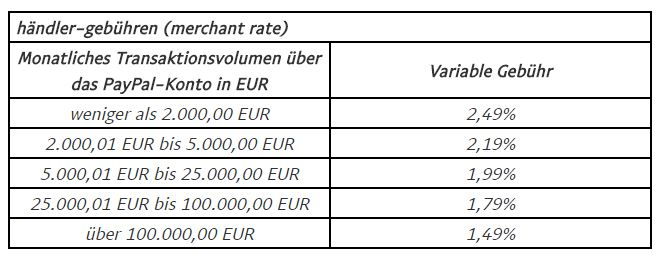
\includegraphics[width=8cm]{media/paypal.png}
        \caption{Paypal's Gebühren}
        \label{gebühren-paypal}
        \bildquelle Paypal erhöht Gebühren für Händler. In: Sellercamp (2019). https://bit.ly/3nWdMna. – aufgerufen am 22. 12. 2020
    \end{center}
\end{figure}

\noindent PayPal versucht eine Alternative zu herkömmlichen Bezahlungsmethoden zu sein, obwohl die Sicherheit und der Service von PayPal auch von anderen Unternehmen geleistet werden kann.

        %\subsection{Auswirkungen auf Konzerne und Umwelt}
        %   <<<<<<< Updated upstream
Auch wenn PayPal seine Vorteile mit sich bringt hat es seine Nachteile. Speziell die weitere Nutzung der Daten, die PayPal generiert, ist fraglich. Dabei sendet PayPal Daten an das US-Heimatschutzministerium die die Daten abgleicht mit möglichen Straftätern oder Terroristen, dabei kann schon der geringste Verdacht zu einer Sperrung des Kontos führen. (https://www.it-recht-kanzlei.de/Brauchen_wir_PayPal.html) Ebenfalls ist das Einfrieren von Konten auch ein großer Nachteil, da eine Vielzahl von Menschen der Geldwäsche von PayPal bezichtigt werden, aber ohne jeglichen Beweis. In beiden Fällen kann man Wiederspruch einlegen, aber man muss Nachweißen das alle Zahlungen legal waren und sich ausweisen können. Bis zu dem Zeitpunkt der Wiedereröffnung des Kontos oder Wiederaktivierung falls der Wiederspruch angenommen worden ist können einige Monate vergehen und man hat absolut keinen Zugriff auf das Geld. Dazu hat man keinen Ansprechpartner in Deutschland für einen Beschwerde, sondern muss sich an die englische Behörde wenden, wodurch auch englisches Recht gilt, dadurch ist das Unternehmen nahezu unantastbar in Deutschland. 
=======




Durch diese Grundstrukturen hat sich ein Wirtschaftssektor gebildet der profitabelste Sektor für ein großes Unternehmen ist. Besonders durch die Einbeziehung des Onlinehandels konnte der E-Commerce erst seinen Aufstieg feiern. Jedoch ist das Potential des Sektors noch lange nicht ausgeschöpft. Durch die Entwicklung von Sprachassistenten und Künstlichen Intelligenzen wird die Zeit des Prozesses des Einkaufens bis zum minimalen verringert. Auch durch das Integrieren von Drohen wird die Allgegenwärtigkeit des Onlinehandels früher oder später offensichtlich. %(https://www.tagesschau.de/wirtschaft/amazon-drohnen-101.html) 
Die Steigerung des Kommerzes, ins besonderen in ländlichen Regionen ist überwältigend. Vom Jahr 2000 bis 2020 hat sich der Umsatz in Deutschland mehr als verfünfzigfacht. Von 1,3 Milliarden € auf 59,2 Milliarden € in nur zwanzig Jahren. %(https://de.statista.com/statistik/daten/studie/3979/umfrage/e-commerce-umsatz-in-deutschland-seit-1999/)
Auch zeigen die tendenzen in den kommenden Jahren nur nach oben. Bis 2023 sollen 71,4 Milliarden € Umsatz im Sektor E-Commerce gemacht werden.       
 
%(https://parcellab.com/wp-content/uploads/2019/09/statistic_id488012_prognose-der-e-commerce-nutzer-in-deutschland-bis-2023.png) 
>>>>>>> Stashed changes

        \newpage
        
        
        
    \section{Onlineversandhändler am Beispiel Amazon} 
         Amazon ist ein Onlineversandhändler, der eine breite Bekanntheit genießt und vor allem im europäischen Raum im Bereich des Onlinehandels einen großen Anteil ausmacht. Während Aliexpress in Asien und östlichen Teilen Europas und Ebay im Norden der EU stark vertreten sind, ist Amazon in Zentral-, Nord- und Westeuropa die Plattform mit dem größten Wert von Verkäufen\cite[S. 22]{EuroCommerce}. Außerdem macht Amazon bereits seit Ende 2017 mehr als die Hälfte der Verkäufe durch Drittanbieter aus\cite[S. 25]{Haendlerbund}. Dementsprechend werde ich in den folgenden Unterpunkten die Firma in Bezug auf ihre Entwicklung, die Auswirkungen dieser und der Konkurrenzfähigkeit zu lokalen Händlern analysieren und auf Basis der Erkentnisse Schlussfolgerungen im Bezug auf Schleusingen und des hildburghäuser Landkreis schließen.

        \subsection{Entstehung und Entwicklung}
            Als Amazon, anfangs noch \emph{cadabra.com}, am 5. Juli 1994 von Jeff Bezos und seiner Frau McKenzie gegründet wurde, hatte wahrscheinlich niemand die Vision eines marktführendem Online-Unternehmens im Kopf - im Gegensatz, Amazon war ursprünglich ein Online-Buchhandel für bestimmte, seltene Bücher\cite[S. 17]{Graf}. Trotz der kleinen Zielgruppe wuchs das Unternehmen in den folgenden Jahren bedeutend: schon zwei Jahre später wurden Aktien angeboten, außerdem wurde anfangs noch fast der komplette Gewinn reinvestiert\cite{Rosoff}, was das Aufkaufen ganzer Unternehmen schon 4 Jahre nach der Gründung ermöglichte, bespielsweise von \emph{pets.com} und \emph{overstock.com}\cite{ChannelAdvisor}. An der Strategie, Unternehmen komplett zu kaufen, hat sich bis heute nichts geändert - im Gegenteil, Amazon kauft heute mehr und größere Unternehmen als je zuvor\cite[S. 27]{Haendlerbund}, wie Audible, Kiva Systems oder Twitch\cite{Sherman}. Der Gewinn wird jedoch nicht mehr ausschließich reinvestiert\cite{Rosoff}. Mit der Zeit expandierte die Firma in viele weitere Gebiete: Cloud Computing mit \ac{AWS} 2002 sowie Musik mit einem Online-Musik-Store und Lebensmittel mit AmazonFresh im Jahr 2007\cite{Sherman, ChannelAdvisor}. Auch bezüglich des Onlinehandels breitete Amazon ab 2000 nach und nach die Produktauswahl aus, wodurch sich der darmalige Buchhandel zu dem heutigen Onlineversandhandel für fast alle Produktereiche entwickelte. Ein wichtiger Schritt zu diesem Ziel war das Ermöglichen von Drittanbieter-Verkäufen ab dem 30. September 1999, was die Bekanntheit und Anzahl der Verkäufe erheblich steigerte\cite{Sherman}. Außerdem wurden weitere Technologien wie Amazon Prime und AmazonBasics entwickelt, die den Onlinehandel und -versand unterstützen\cite{ChannelAdvisor}, aber auch alleinstehende Projekte, wie Kindles, das Fire Phone oder Smart-Home-Geräte\cite{Sherman}.

Die derzeitige Strategie bezüglich des Oninehandels beschrieb Bezos, als "Virtuos Cycle" betitelt, schon 2001  mit folgender Zeichnung\cite{zentail}:
%IST NICHT IMMER DA WO ES SOLL WENN ES ZB NICHT AUF DIE SEITE PASST
\begin{figure}[h]
    \begin{center}
        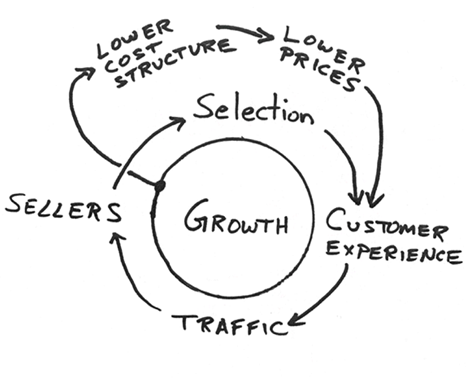
\includegraphics[width=8cm]{media/Fabian-vicious-cycle.png}
        \caption{Amazon's Vicious Cycle}
        \label{vicious-cycle}
        \bildquelle Jeff Bezos, September 2001 %Learn from the Bezos Virtuous Cycle: Leverage and Invest in Infrastructure, www.zentail.com, abgerufen August 2020% https://tinyurl.com/yyu2zz29 DATUM???
    \end{center}
\end{figure} 

Dabei schafft breit gefächerte Produktsegment(Selection) eine positive Kundenerfahrung(Customer Experience), die weitere Verkäufe und Verbreitung durch z. B. Empfehlungen(Traffic) hervorruft. Durch diese hohe Kundenanzahl ist die Plattform wiederrum attraktiver für Drittanbieter und Herstellern(Sellers), die weitere Produkte anbieten und das Produktsegment erweitern. Dieser Teil ist an sich nicht wirklich außergewöhnlich, da viele andere Onlineanbieter eine ähnliche Strategie verfolgen. Jedoch hebt sich Amazon damit ab, ungewöhnlich hohe Summen zu investieren, um Kosten(Lower cost structure) und somit auch Produktpreise(Lower prices) zu senken\cite[S. 26f]{Graf}. Amazon schaffte so auch ein neues Kundenverhalten, das "Amazon Commerce" - Graf und Schneider beschreiben es in ihrem Buch als ein

\begin{quote}
    "[...] komplett neues Kaufverhalten, das sich nicht mehr an Anbietern oder konkreten Produkten orientiert, sondern allein am Zweck [...], den das gewünschte Produkt erfüllen soll."\cite[S. 42]{Graf}
\end{quote}

Die genannten Punkte ermöglichten es Amazon, sich als weltweit bekannten und benutzten Onlineversandhandel zu etablieren - jedoch haben sie auch einige Probleme hervorgerufen. Beispielsweise führte die konstante Niedrigpreispolitik\cite[Abb. 5]{Desjardins} zum Einsparen von Ausgaben in fast allen Gebieten - auch im Bezug auf Angestellte\cite[S. 6]{Apicella}. \iffalse Amazon’s Haupteinnahmequelle ist mit 84\% der Einnahmen zweifelsfrei der Onlinehandel und -versand\cite[Abb. 5]{Desjardins} - und genau dieser hat in den letzten Jahren einige Probleme hervorgerufen. Bespielsweise führt die Verkauffstrategie Amazons, Produkte so billig wie möglich und mit kostenlosem Versand anzubieten, um mehr Käufer anzusprechen\cite{Quartz}, zum Einsparen von Ausgaben in fast allen Gebieten - auch im Bezug auf Arbeiter\cite[S. 6]{Apicella}.\fi So werden insbesondere in der Weihnachtszeit Leiharbeiter eingestellt. In der ARD-Reportage "Ausgeliefert! Leiharbeiter bei Amazon" wird 2013 gezeigt, wie deren Arbeitsalltag aussah: Zu siebt wird in einer Ferienwohnung übernachtet, oft bekommen die Angestellten nur wenige Stunden Schlaf. Jeden Tag aufs neue ist es unsicher, ob man gebraucht wird - wenn nicht, gibt es keinen Lohn. Mitarbeiter der Dienstleistungsgewerkschaft Ver.di und Amazons erklären, dass 2013 in Koblenz circa 3100 von 3300 Arbeitern befristet angestellt waren\cite{Ausgeliefert}.
Außerdem existiert ein hoher Grad an Überwachung und Kontrollen, wie Apicella in ihrer Studie andhand der Stadt Leipzig beschreibt\cite[S. 29]{Apicella}:
\begin{quote}
"Die Verkaufsarbeit durchläuft dabei einen Prozess der [...] vollständige[n] Überwachung und Disziplinierung der Beschäftigten[...]."
\end{quote}
Dementsprechend sind Streiks bei Amazon keine Seltenheit: Beispielsweise streikten Angestellte in Deutschland zwei Monate nach der besagten Reportage unter dem Motto "Wir sind keine Roboter" gegen niedrige Löhne, befristete und schlechte Arbeitsverhältnisse sowie die starke Digitalisierung der Arbeit\cite[S. 6]{Apicella}. Amazon reagierte in den folgenden Jahren mit mehreren Lohnerhöhungen, jedoch exestieren noch vereinzelt Streiks\cite{JGraf}.

Da in Folge der Corona-Krise im 1. Quartal von 2020 die Verkäufe um 32\% stiegen, bekamen Angestellte eine weitere Lohnerhöhung. Zusätzlich wurden 175000 neue Stellen ausgeschrieben - nicht nur, weil mehr Arbeiter als vorher gebraucht werden, sondern auch weil einige Angestellte aufgrund von "unsicheren Bedingungen" zu Hause geblieben sind bzw. dies immer noch tun\cite{Theweek}.

Innerhalb der letzen 26 Jahre hat Amazon sich von einem Online-Buchhandel zu einem weltweiten Onlinehändler fast alle Produktklassen entwickelt. Außerdem bietet die Firma heute auch andere Dienste an, wie z. B. Cloud Computing mit \ac{AWS}. Jedoch steht das Unternehmen bezüglich der Arbeitsbedingungen seit fast einem Jahrzehnt in der Kritik.

%dritanbieter: so kann amazon ein noch breeiteres produktsegment anbieten, während probleme wie kapitalbildung und lagern an händler auszulagern + provision: ecom Buch S 50

            
        \subsection{Einfluss auf das Konsumverhalten } %neu: das Konsumverhalten und der Einfluss des Onlinehandels
            Der Ablauf von Kaufprozessen hat sich in den letzten Jahrzehnten unter Einfluss des Onlinhandels stark geändert. Insbesondere Amazon hat sich als Händler mit niedrigen Preisen und einer sehr großen Auswahl von neuen sowie gebrauchten Produkten weltweit als Verkaufsplattform etabliert. Mithilfe dieser Kombination kann Amazon, im Gegensatz zu anderen Plattformen wie Ebay als Haupteinkaufsmöglichkeit benutzt werden, was wiederrum anderer Online-Konkurrenz und dem stationären Einzelhandel schadet.


%Neben Ebay, welches sich ausschließlich auf Drittanbieter fokussiert, konnte sich nur ein anderes Unternehmen im Onlineverkauf aller Branchen etablieren: Abiexpress, welches noch niedirgere Preise durch Direktverkauf von Herstellern ermöglicht. \emerald 345
Der Hauptgrund für diesen Wandel ist wahrscheinlich, dass bei den meisten Verbrauchsgütern die in [4] beschriebenen Vorteile des stationären Handels\cite[S. 2]{Maier}, hauptsächlich die Beratung und das direkte Betrachten des Produktes, nur wenig Nutzen finden. So ist z. B. beim wiederholten Kaufen von Shampoo, Rasierklingen o. ä. das Produkt schon bekannt und kann problemlos Online bestellt werden. 

\iffalse
    über zeit unkomplizierter geworden
    
    verbilligung des onlinehandels > prime-verlust
    amazon = vorreiter, aliexpress
    
    aliexpress: direkt von hersteller kaufen (https://www.emerald.com/insight/content/doi/10.1108/S1745-886220180000013014/full/pdf?title=italicamazon-and-alibabaitalic-internet-governance-business-models-and-internationalization-strategies 345)
\fi
Dementsprechend führt die seit Jahrzehnten steigende Relevanz des Onlinehandels zu einem Rückgang der Nachfrage im stationären Vertrieb\cite{Shankar}, die durch die derzeitige Corona-Situation noch etwas verstärkt wird - mehr dazu in Kapitel [4 und 5].

\iffalse
 Vorreiter in sachen niedrige Preise > ist sehr wichtig, weil
   viel einfacher vergelichbar, qualität des Produkts nicht einfach einsehbar: sie muss nicht außergewöhnlich, nur akzeptabel sein - jedoch auch nicht schlecht, da 14-tage-rückgabe ohne angabe eines grundes

 
 S 49 https://edoc.sub.uni-hamburg.de/hcu/volltexte/2017/370/pdf/Ebert_Kirsten.pdf
 danach: modell für veränderung
\fi

        \newpage
            
            
        
    \section{Globaler Vergleich des Einflusses und der Entwicklung des Onlinehandels}
            \iffalse

deu: 14-tage rückgabe durch §355 BGB

\fi

        \newpage
        
        
        
    \section{Ergebnisse}
        \subsection{Zusammenfassung}
            \subsubsection{Konsumentenperspektive}
asldfjjsdalfjlsdajfldsf
 

%ergenisse: nischenwaren mit onlineversand, oder online-verbund mit anderen\ nitt 63
    %viele einzelhandelsflächen ini der stadt durch insolvenzen
    %mglich: hersteller-fabrik einige km von stadtzentrum, laden in der stad, mit onlineshop
    %stärkere, individiuelle bedürfnisse
    %standort immer wichtiger, am besten shoppingcenter \nitt, 7
    %handwerker, baumarkt, apotheken
    %lebensmittel-liefer-roboter zwar in zukunft denkbar, jedoch noch nicht umsetzbar weil probleme wie vandalismus(unbegründete zerstörung von dingen)
    %stationärer handel hat in vielen gebieten geringe zukunftschancen: er wird zwar überleben, trotzdem ist der einstieg neuer händler um so schwerer - jedoch wird er für eine interesannte innenstadt nicht benötigt
    %attraktionen statt verkauf: zB lasertech
    %oder Gastronomie- und Dienstleistungsangebote (zum Beispiel Frisör, Reinigung, Krankengymnastik, Arztpraxen)
    % oder Bildungs- oder Kulturangeboten wie fahrschule

             
\subsubsection{Einschätzung der Thesen}

Die Existenz des Distanzhandels verringert bereits seit seiner Entstehung die Nachfrage des stationären Handels in fast allen Produktgruppen, und führt damit zu stationären Umsatzeinbußen. Infolgedessen haben stationäre Händler - insbesondere im ländlichen Bereich, da hier aufgrund einer niedrigeren Bevölkerung pro Vertrieb eine allgemein geringere Nachfrage vorherrscht - deutlich schlechtere Chancen, ihr Geschäft Umsätze erzielen zu lassen, insbesondere falls Güter außerhalb der Produktgruppe der \ac{FMCG} verkauft werden. Dementsprechend können derzeit deutlich mehr Insolvenzen stationärer Vertriebe beobachtet werden und die These "Der Onlinehandel führt zu einem allmählichen Aussterben von stationären Händlern im ländlichen Bereich." verifiziert werden.

Jedoch muss dabei auch bzgl. der Gütergruppen differenziert werden - zwar können alle Güter mit mehr oder weniger Nachteilen online gekauft werden, jedoch ist der Aufwand und weitere negative Einflüsse des Onlinehandels bei einigen Produkten so relevant, dass diese fast ausschließlich stationär gekauft werden, wie beispielsweise Nahrungsmittel. Dementsprechend kann auch die These, dass es Waren gibt, die nicht online gekauft werden, bis auf einige Ausnahmefälle bestätigt werden.

Bei Betrachtung der Arbeitsverhältnisse ist eine eindeutige Einordnung der These, dass durch den Onlinehandel weniger Arbeitsplätze geschaffen werden als indirekt verringert werden, kaum möglich. Einerseits verlieren stationäre Händler an Relevanz und können folglich weniger Arbeitnehmer beschäftigen, jedoch werden, um die Funktionalität des Distanzhandels zu gewährleisten, auch mehr Arbeiter gesucht - insbesondere für Lager- und Transportverwaltung. Außerdem ist das Aussterben von Innenstädten nicht ausschließlich durch den Onlinehandel begründbar, sondern zu einem großen Teil auch durch eine 
\begin{quote}
"grundsätzliche Verschiebung in den Handelsmodellen" \cite[S. 24]{evilcom}.
\end{quote}
Demnach kann die genannte These weder falsifiziert noch verifiziert werden.

Die vierte These, die im Rahmen dieser Arbeit untersucht wird, beschreibt dass durch den Onlinehandel eine zunehmende Umweltbelastung entsteht. Dies ist in erster Linie anhand einem erhöhtem Verkehrsaufkommen durch dass parallele Nutzen von Online- und Offlinehandel problemlos verifizierbar - jedoch könnte in einer fernen Zukunft, in der nahezu ausschließlich der Vertriebsweg des Distanzhandels genutzt wird, sogar eine Kraftstoffersparnis, die in Kapitel 4.1.2 beschrieben wird, erreicht werden.

        \subsection{Schlussfolgerungen im Bezug auf Schleusingen}
            Die bereits genannten Ergebnisse können nahezu ausschließlich auf die Kleinstadt Schleusingen übernommen werden, jedoch bestehen bzgl. der Verkaufsgebiete auch einige Besonderheiten.

Schleusingen bildet im Vergleich zu vielen Städten ähnlicher Größe einen Sonderfall: durch das Einkaufszentrum "Megacenter Schleusingen GmbH" in der Suhler Straße ist hier eine Güterbeschaffung auch für Bewohner der Dörfer um Schleusingen mit vergleichsweise hoher Auswahl möglich - was dem stationären Einzelhandel zugute kommt. Händler können hier auf Kosten von höheren Ausgaben besser wahrgenommen werden und eine erhöhte Nachfrage erfahren. 

Auch das Gebiet in der Nähe des hennebergischen Gymnasiums "Georg Ernst" und um den Markt haben eine nachfragetechnische Besonderheit: Schüler des Gymnasiums - insbesondere die der oberen Klassen - kaufen hier nach der Schule oder in Pausen oft ein. Für neue Geschäfte empfehlen sich besonders Frisch- und Fertingnahrungsmittelverkäufer, die den Verkaufsraum von heute nicht mehr vorhandenen Geschäften wie Mode Beetz nutzen können. Jedoch ist darauf zu achten, das sich das Verkaufsangebot nicht mit dem bereits vorhandenen überschneidet: Fleischer und Bäcker sind zu genüge vorhanden, jedoch nicht etwa ausgefalleneres wie Fischspezialitäten. Auch jugendorientierte Unternehmen könnten hier einen stationären Vertrieb gewinnbringend betreiben - vorausgesetzt, die nötige Nachfrage ist vorhanden.

Eine weitere Besonderheit bildet das Gebiet um die staatliche Grund- und Regelschule "Gerhart Hauptmann": Hier können Händler ähnlich wie Verkäufer in der Nähe des Gymnasiums einen nachfragetechnischen Vorteil erlangen, jedoch ist hier nur schwierig eine mögliche Fläche zu erhalten.

Abschließend ist anzumerken, dass die Standortwahl eines stationären Unternehmens von unzähligen Faktoren abhängt - so können beispielsweise durch den Onlinewandel nur noch wenige stationäre Vertriebe bestehen. Wir können im Rahmen dieser Arbeit zwar auf solche Besonderheiten hinweisen, jedoch keine Entscheidung abnehmen. 

% hängt von vielen faktoren ab, ich möchte nicht herausnehmen unternehmen die entscheidung abzunehmen

% markt mit schule, regelschule ungünsitg wegen baufläche

        \newpage
        
        
        
    \bibliography{Literaturverzeichnis}
        \newpage
        
    \listoffigures
        \newpage
        
    \input{exports/Abkürzungsverzeichnis.tex}
    
    %\listoftables
    %    \newpage
    \addsec{Materialanhang}
        \newpage
    
    \addsec{Auswertung der Schülerumfrage}
\normalsize
Im Zeitraum vom 17. 11. 2020 bis 26. 11. 2020 führte unsere Seminarfachgruppe eine anonyme Online-Umfrage für Schüler des hennebergischen Gymnasiums "Georg Ernst" durch. Jegliche erhobenen Daten wurden ausschließlich im Rahmen dieser Arbeit benutzt und nach der entsprechenden Auswertung gelöscht. Zum Zeitpunkt der Auswertung haben insgesamt 147 Schüler teilgenommen.\\\\
Wenn mehrere Antworten angegeben wurden, zählt jede je nach Frage entweder als eine Stimme(*) oder eine Stimme wird anteilmäßig auf die genannten Antwortmöglickeiten verteilt(**).\\\\\\\\\\\\\\\\



Würden Sie die folgenden Produkte eher Online oder vor Ort kaufen? (1)\\\\
\begin{figure}[H]
    \begin{center}
        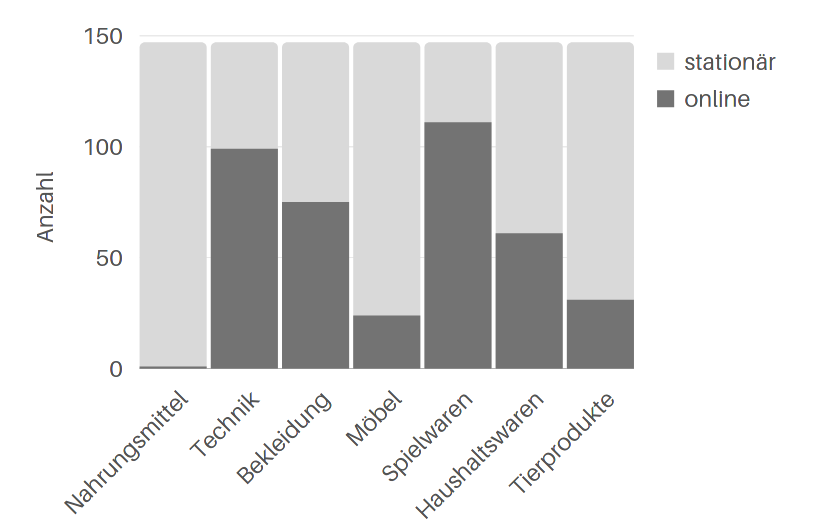
\includegraphics[width=12.5cm]{media/schuelerumfrage/1.png}
    \end{center}
\end{figure} 



\newpage\noindent Haben Sie schon einmal etwas Online bestellt, wenn ja über welche Plattform? (2)\\
\begin{figure}[H]
    \begin{center}
        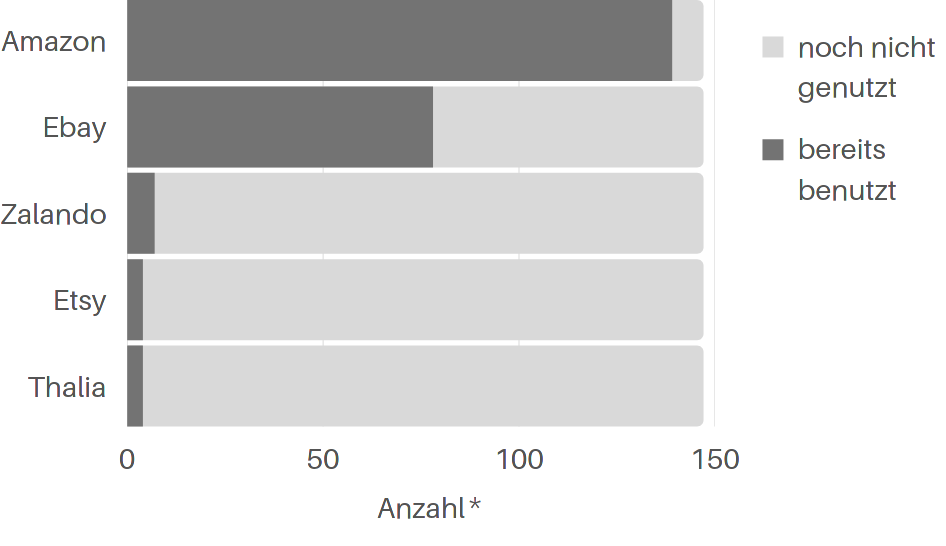
\includegraphics[width=11.5cm]{media/schuelerumfrage/2.png} 
    \end{center}
\end{figure}

\noindent weitere genannte Plattformen:
\begin{itemize}
 \item Zaful (3)
 \item H\&M (2)
 \item EMP (2)
 \item Intersport (2)
 \item Bershka (1)
 \item Shein (1)
 \item Maciag Offroad (1)
 \item Reifendirekt (1)
 \item Böttcher AG (1)
 \item Globetrotter (1)
\end{itemize}



\iffalse \newpage\noindent Gibt es Artikel, die Sie nicht Online bestellen würden?** (3)\\\\\\
\begin{figure}[H]
    \begin{center}
        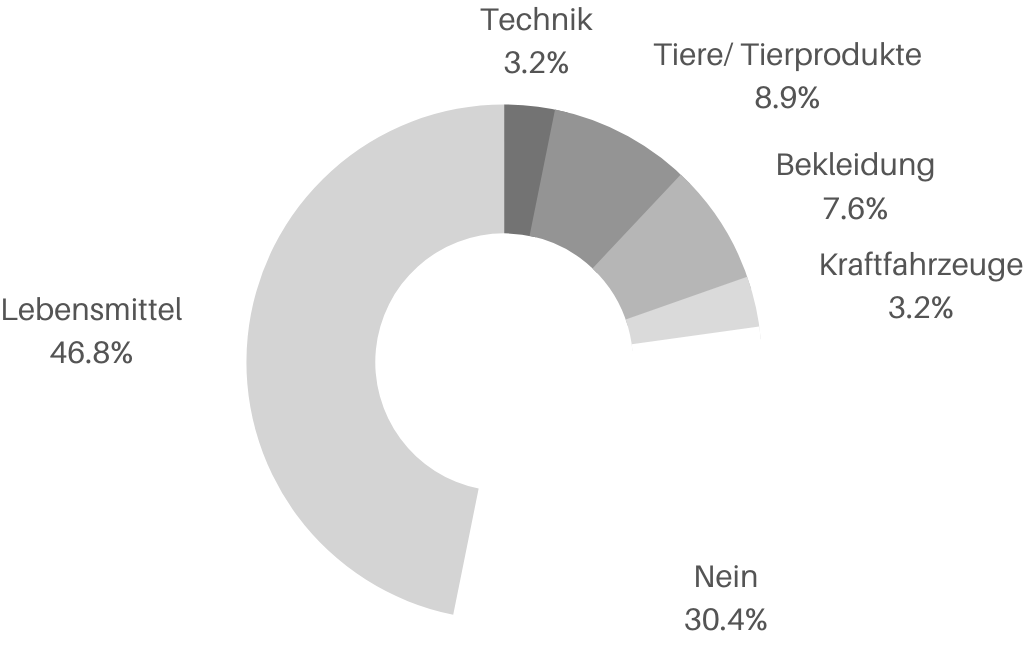
\includegraphics[width=11.5cm]{media/schuelerumfrage/3.png}
    \end{center}
\end{figure}
\vfill
\noindent weitere genannte Produkte:
\begin{itemize}
 \item Gebrauchtwaren (3)
 \item Mietwohnung (1)
\end{itemize}
\vfill\vfill\vfill\vfill \fi



\iffalse \newpage\noindent Wie beschreiben Sie ihre Erfahrungen mit dem Onlinehandel? (4)\\\\\\
\begin{figure}[H]
    \begin{center}
        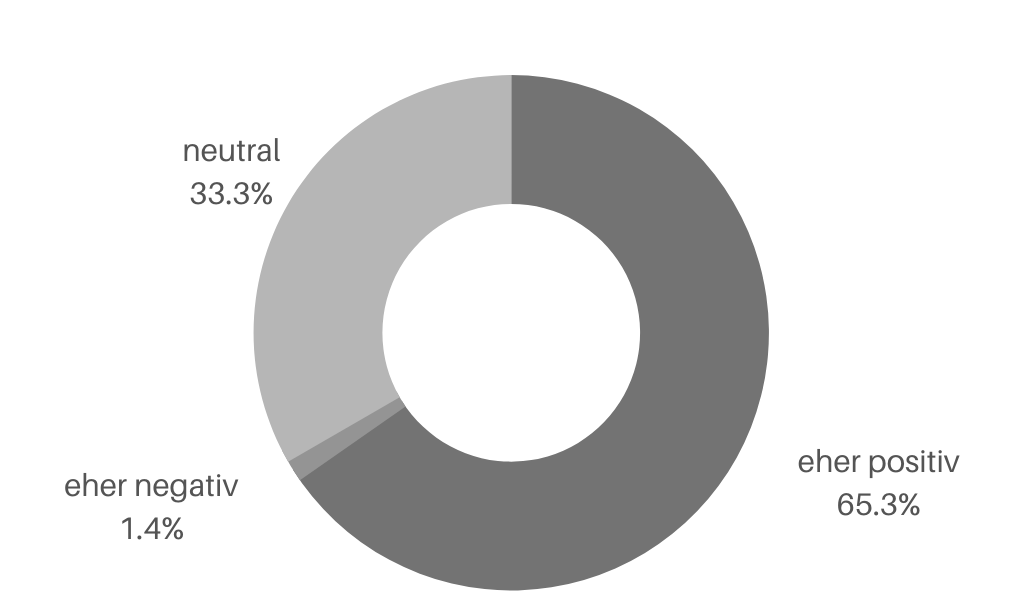
\includegraphics[width=11.5cm]{media/schuelerumfrage/4.png}
    \end{center}
\end{figure} \fi



\iffalse \newpage\noindent Ist das Kaufangebot im schleusinger Umkreis ausreichend? Falls nein, was fehlt?** (5)\\
\begin{figure}[H]
    \begin{center}
        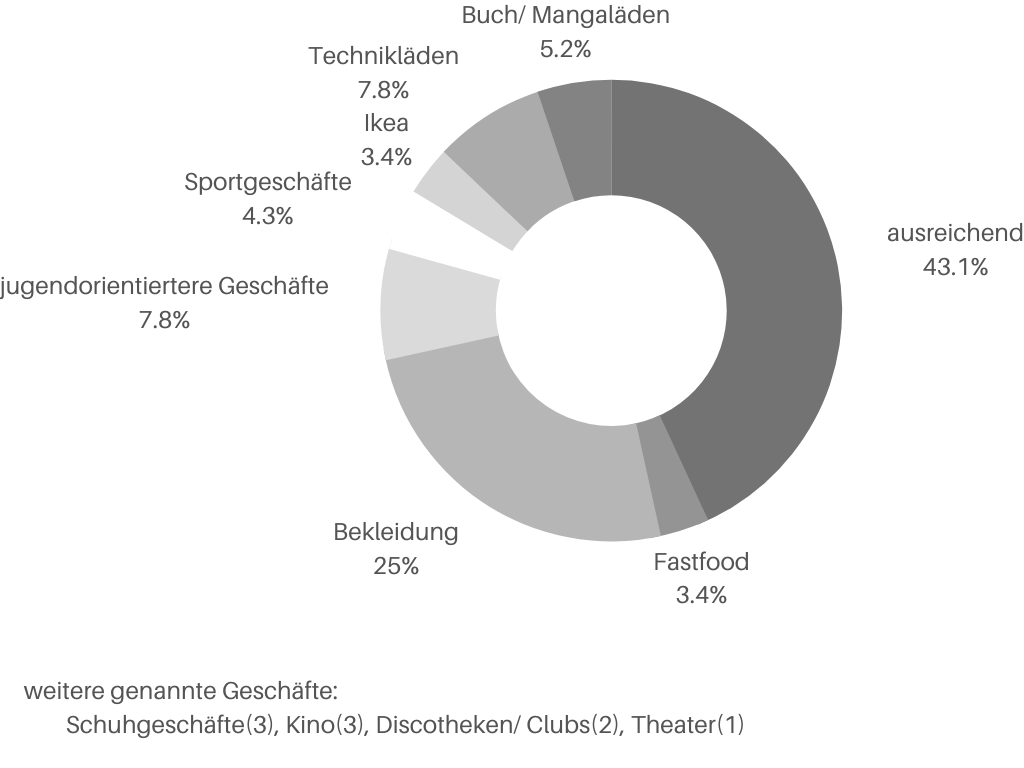
\includegraphics[width=15cm]{media/schuelerumfrage/5.png}
    \end{center}
\end{figure} \fi



\newpage\noindent Weichen Sie und ihre Familie beim Einkaufen aufgrund des Angebots auf andere Städte in der Umgebung aus? (6)\\
\vfill
\begin{figure}[H]
    \begin{center}
        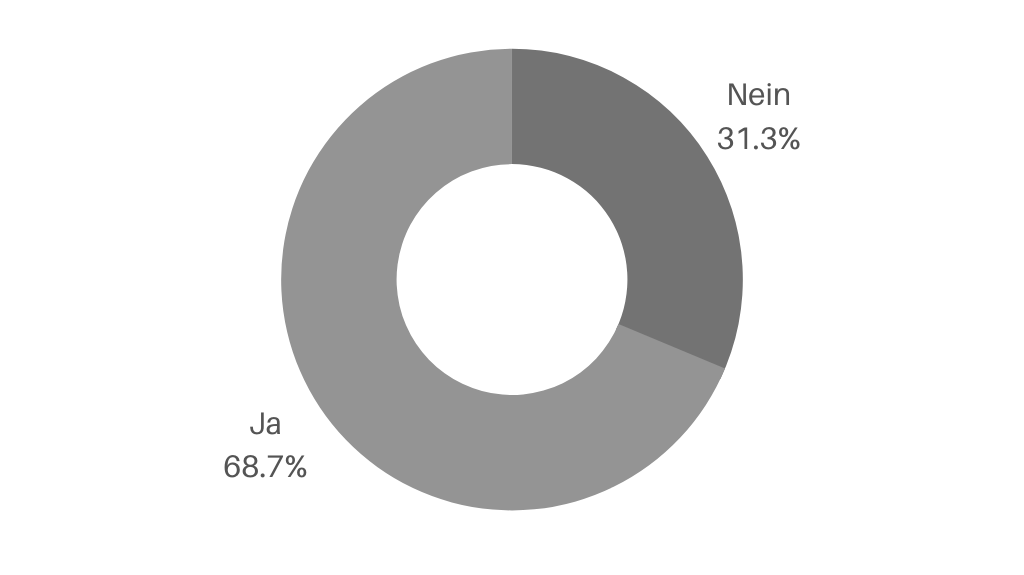
\includegraphics[width=12cm]{media/schuelerumfrage/6.1.png}
    \end{center}
\end{figure}
\vfill
\begin{figure}[H]
    \begin{center}
        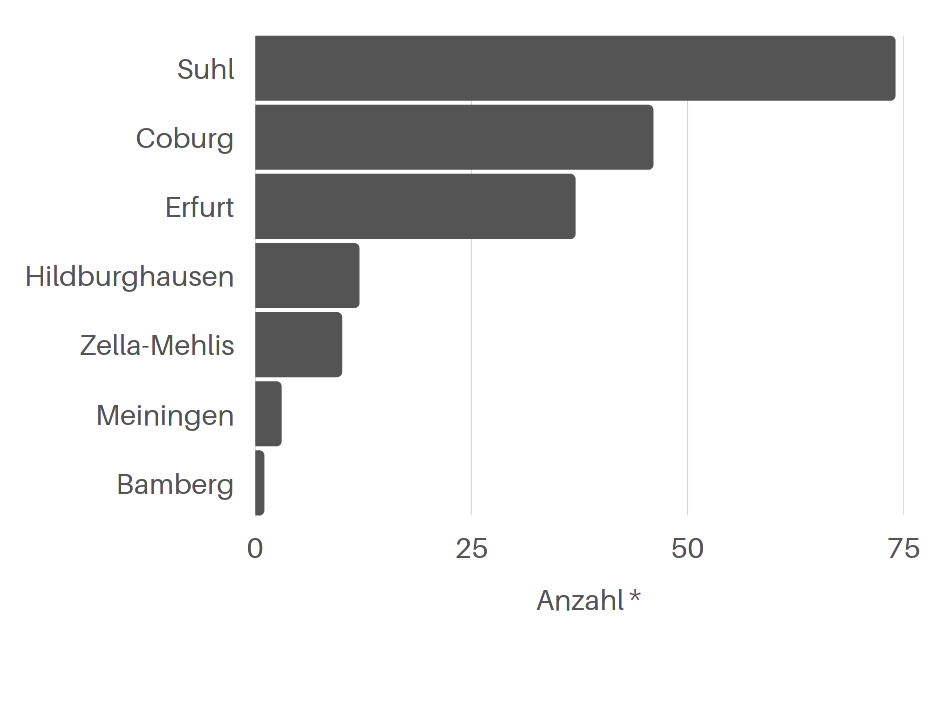
\includegraphics[width=12cm]{media/schuelerumfrage/6.2.png}
    \end{center}
\end{figure}
\vfill



\newpage\noindent Welche Produkte/ Änderungen im Verkaufsprozess wünschen Sie sich für den Onlinehandel? (7)\\\\

\begin{figure}[H]
    \begin{center}
        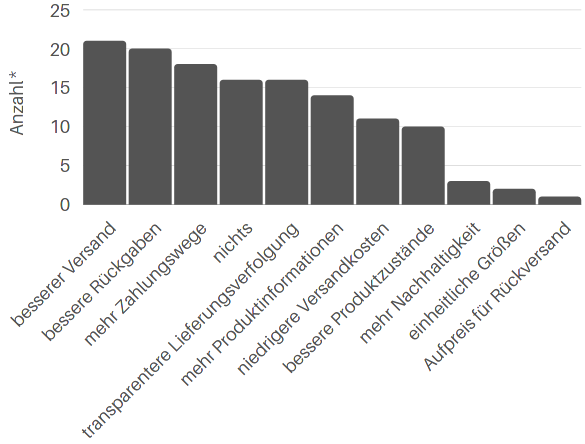
\includegraphics[width=12cm]{media/schuelerumfrage/7.png} 
    \end{center}
\end{figure}
\vfill\vfill
\noindent Auffälligkeiten:
\begin{itemize}
 \item Paypal ist als Zahlungsweg am meisten gefragt
 \item Aufpreis für Rückversand, um Umweltbelastung zu verringern
 \item oft online-spezifisches und geringe Schnittmenge mit Frage 8
 \end{itemize}
\vfill\vfill\vfill\vfill



\newpage\noindent Welche Produkte/ Änderungen im Verkaufsprozess wünschen Sie sich für den lokalen Handel? (8)\\
\vfill
\begin{figure}[H]
    \begin{center}
        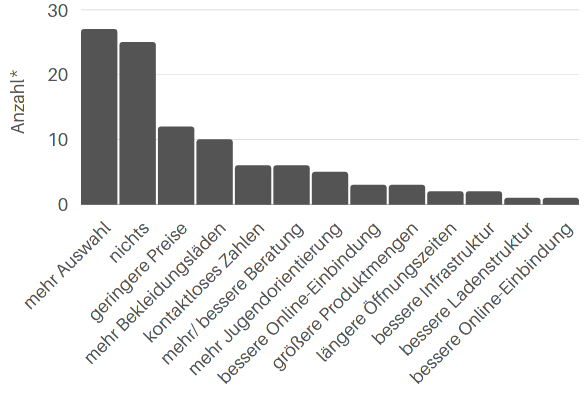
\includegraphics[width=12cm]{media/schuelerumfrage/8.png}
    \end{center} 
\end{figure}
\vfill\vfill
\noindent Auffälligkeiten:
\begin{itemize}
 \item sehr oft "keine Ahnung"
 \item ausschließlich eine größere Auswahl wird oft genannt
 \item wenig bis keine Überschneidung mit Antworten aus Frage 7
 \end{itemize}
\vfill\vfill\vfill\vfill



\iffalse \newpage\noindent Welche Stärken sehen Sie bzgl. des stationären Einzelhandels im ländlichen Bereich? (9)\\
\begin{figure}[H]
    \begin{center}
        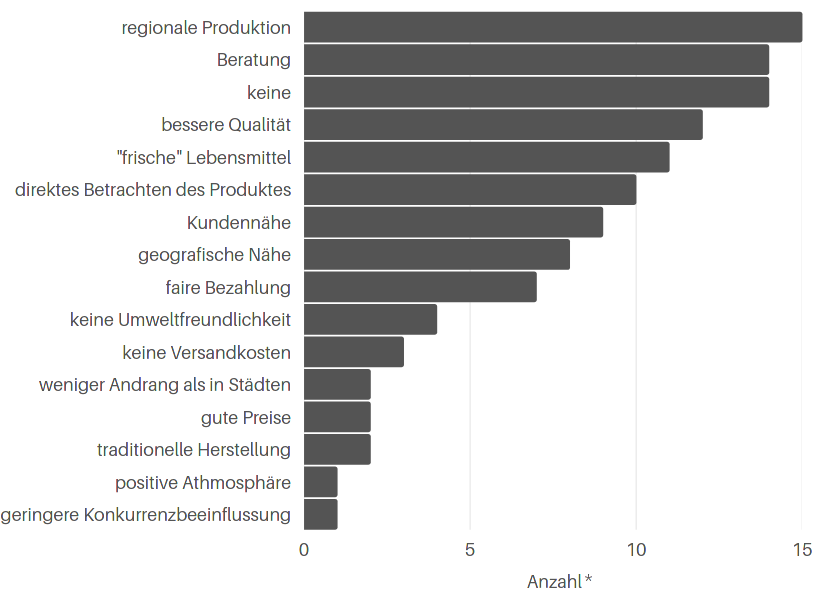
\includegraphics[width=15cm]{media/schuelerumfrage/9.png}
    \end{center}
\end{figure} \fi



\iffalse \newpage\noindent Kaufen Sie und ihre Familie Gebrauchsgegenstände (mehrfach verwendbare, z. B. Autos, Fernseher usw.) größtenteils neu oder gebraucht? (10)\\

\begin{figure}[H]
    \begin{center}
        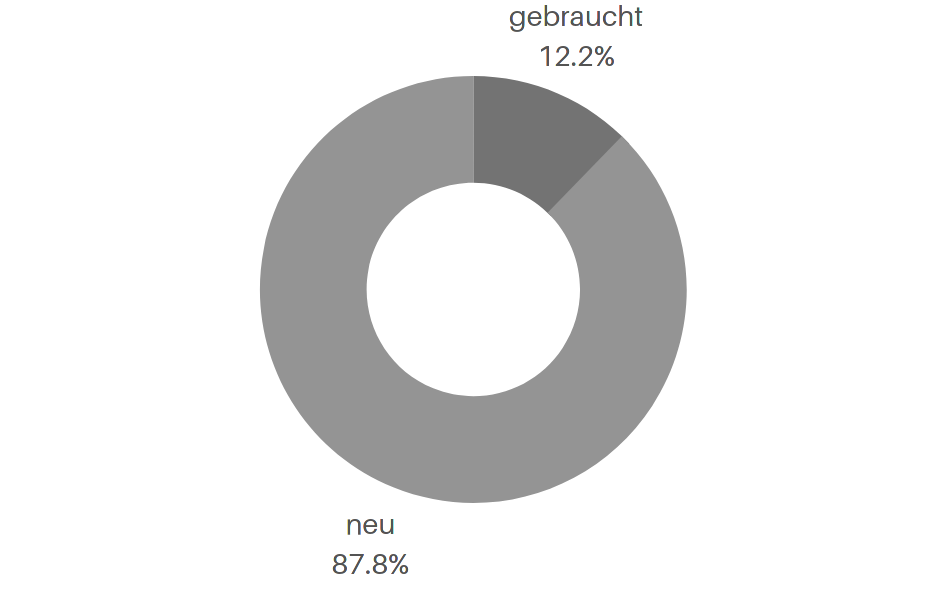
\includegraphics[width=12cm]{media/schuelerumfrage/10.png}
    \end{center}
\end{figure} \fi



\iffalse \newpage\noindent Was ist für Sie relevanter? Der Onlinehandel oder der stationäre Einzelhandel? (11)\\

\begin{figure}[H]
    \begin{center}
        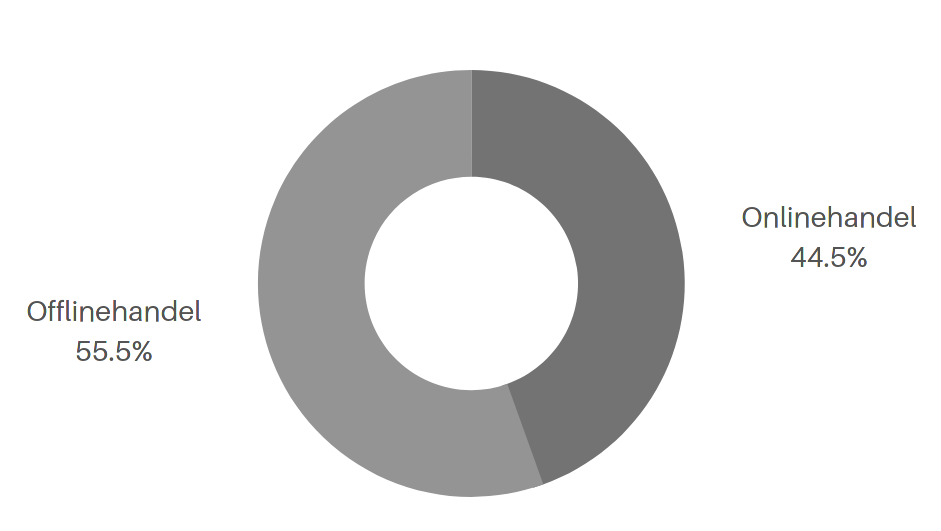
\includegraphics[width=12cm]{media/schuelerumfrage/11.png}
    \end{center}
\end{figure} \fi



\iffalse \newpage\noindent Welche Probleme/ Komplikationen sehen sie beim Kauf von Artikeln Online? (12)
\begin{figure}[H]
    \begin{center}
        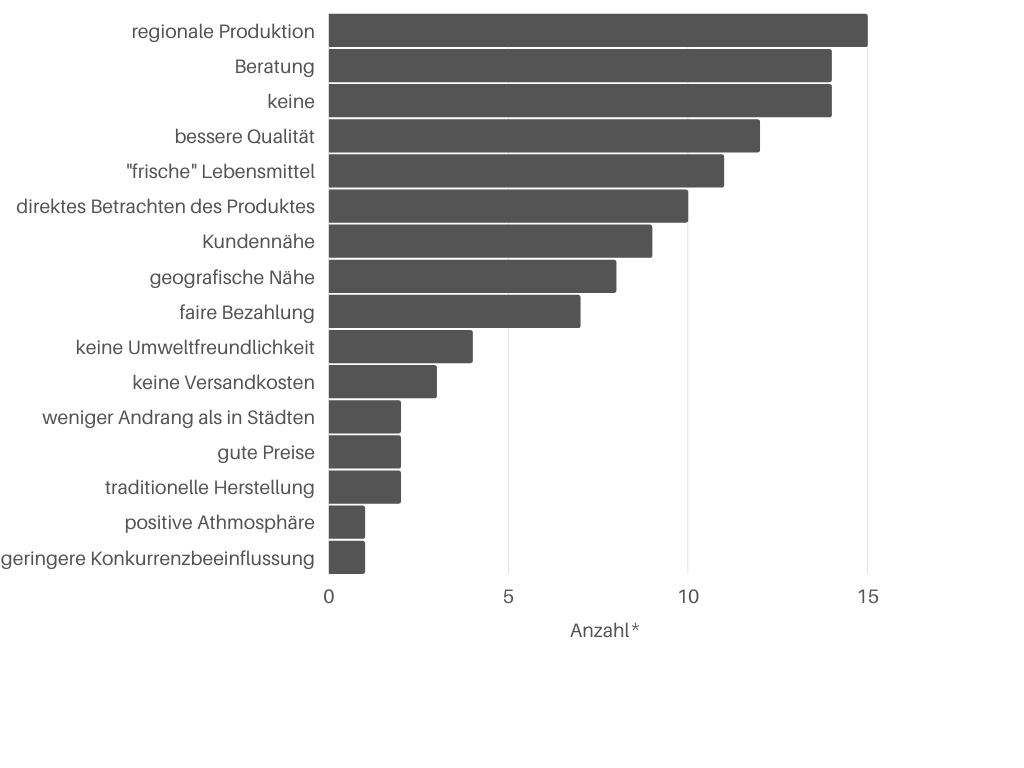
\includegraphics[width=17cm]{media/schuelerumfrage/12.png}
    \end{center}
\end{figure} \fi



\iffalse \newpage\noindent Wie schätzen sie ihre Preissensibilität ein? (13)\\
 
\begin{figure}[H]
    \begin{center}
        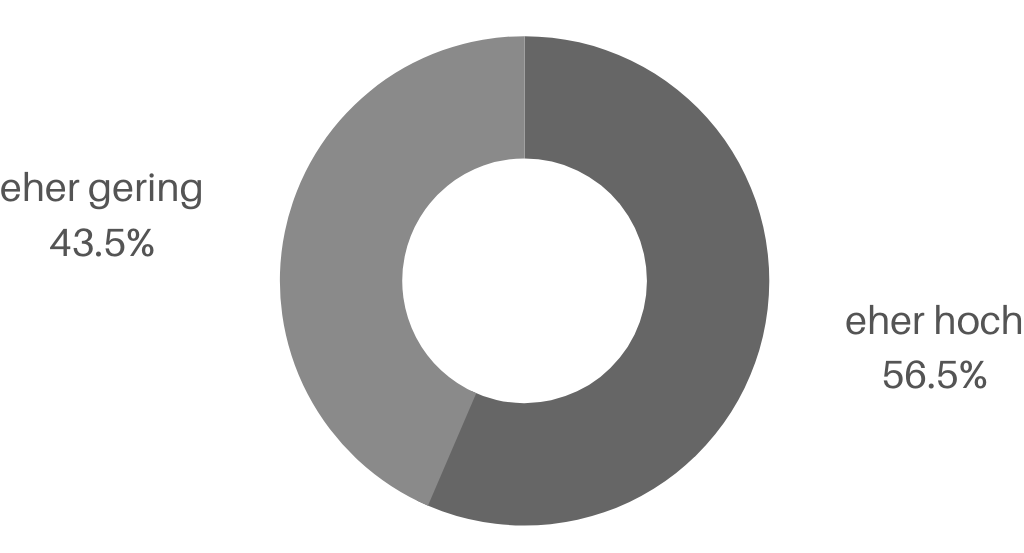
\includegraphics[width=9cm]{media/schuelerumfrage/13.png}
    \end{center}
\end{figure} \fi 



\newpage\noindent Haben sich ihre Kaufgewohnheiten während der Corona-Zeit geändert? (14)\\\\\\

\begin{figure}[H]
    \begin{center}
        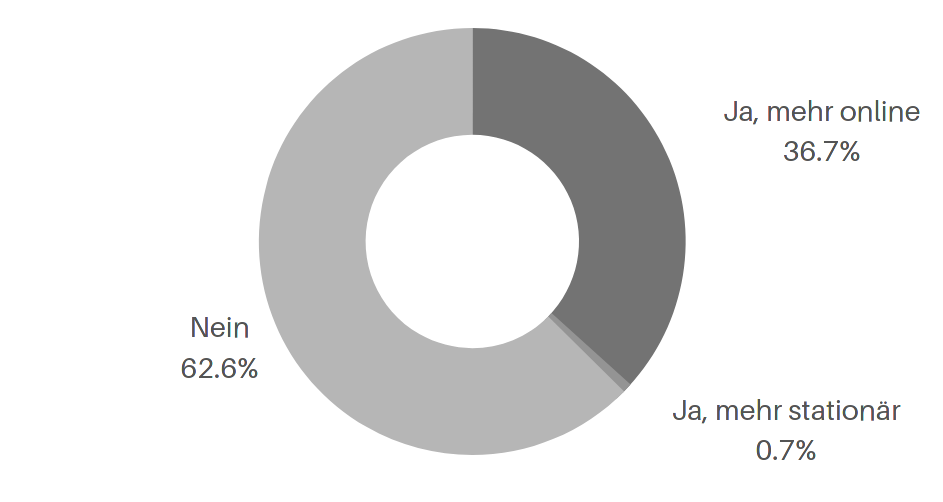
\includegraphics[width=12cm]{media/schuelerumfrage/14.png}
    \end{center}
\end{figure}

\iffalse \noindent Wann haben Sie das erste mal etwas online gekauft? (15)\vfill

\begin{figure}[H]
    \begin{center}
        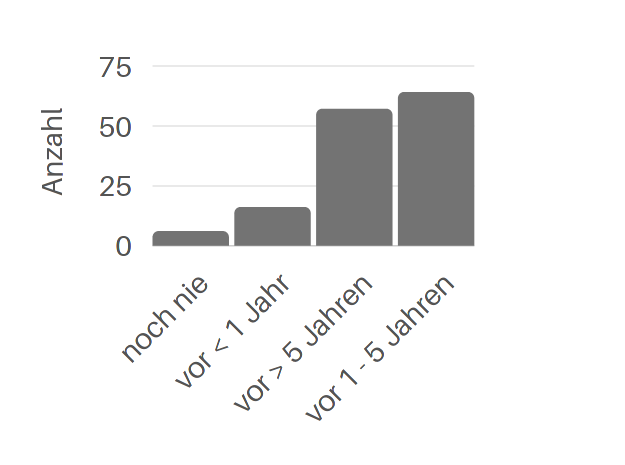
\includegraphics[width=8cm]{media/schuelerumfrage/15.png}
    \end{center}
\end{figure} 
\vfill \fi
\newpage










    \addsec{Interviewtranskript}
Interviewpartner: Prof. Dr.-Ing. André Spindler\\
Datum: 19. 09. 2020\\
Ort: Erfurt\\\\
00:00:00 - 00:40:19\\

\footnotesize
\setspeaker{Andre}[Prof. Spindler]
\setspeaker{Fabian}[Fabian Beez]
\setspeaker{Toni}[Toni Hausdörfer]
\addtolength{\transcriptlen}{1em}

\begin{description}

\Fabian Wir führen jetzt ein Interview mit André Spindler. Er ist selbständiger Architekt und leitet sein eigenes Architekturbüro mit Spezialisierung auf Brandschutz. Möchten Sie hierzu noch etwas ergänzen? \#00:00:26\#

\Andre Ja, vielleicht zu meiner Person. Ich bin über die 60 weg und habe eine fast 40 jährige Berufserfahrung und hab als Bauingenieur studiert, bin jetzt Architekt seit vielen Jahren und habe mich in das Nischendasein eines Brandschutzfachingenieurs hineingearbeitet. Prüfe dort auch das, was andere machen im Auftrag der Landratsämter und berate sehr viel auf dem Gebiet und hab daneben noch eine Professur an der Fachhochschule Erfurt für Baukonstruktion. \#00:01:05\#

\Fabian Denken Sie, dass die Spezialisierung auf ein Gebiet im Bereich Architektur effektiver ist als sein Wissen breit zu fächern? \#00:01:17\#

\Andre Oh, das ist eine ganz interessante Frage, denn ich kann mich noch gut erinnern an meinen Professor, der gesagt hat "Spindler, gehen Sie erst mal in die Breite. Gucken Sie auf allen Gebieten, was es da gibt. Und wenn Sie das spüren in sich nach einigen Jahren, dann gehen Sie in die Tiefe. Nehmen Sie also ein Spezialgebiet und werden Sie auf dem Gut". Und ob ich das nun bewusst gemacht habe, weiß ich nicht. Aber zumindest ist es bei mir so passiert, dass ich auf eine Vielzahl ganz unterschiedlicher Fachgebiete zurückgreifen kann, in meiner Spezialtätigkeit, und da sich dieses System, überall ein Stück zu wissen, aber auf einem Gebiet sehr viel zu wissen für mich als sehr gut herausgestellt hat. \#00:02:01\#

\Fabian Wie sieht Ihr durchschnittlicher Arbeitsalltag aus? \#00:02:11\#

\Andre Das ist eine ganz schlimme Frage, weil in der Arbeitsbelastung ist man allgemein als Selbstständiger sehr hoch belastet. Und bei mir durch diese mehreren Standbeine und Tätigkeiten ist es deutlich höher als im Durchschnitt. Ich habe also zwei Tage die Woche, in denen ich an der Hochschule tätig bin, mich mit Vorlesungen, Seminaren beschäftige, studentische Fragen beantworte und mehrere Tage die Woche, wo ich mich um mein Büro kümmere und auf Baustellen unterwegs bin. Und oftmals ist es eben das Wochenende, wo ich mich dann um Abrechnungen kümmere, um spezielle Aufgaben, die man als Büroleiter von zehn Beschäftigten hat, am Monatsende Abrechnungen zu machen und ähnlichem. Also der Arbeitstag ist mehr als voll - etwas, was ich am Anfang dieser ganzen Tätigkeiten auch nicht so geahnt habe, dass es so viel Arbeit ist. Ich kann dir aber nicht abwählen, die ist nun mal da. Sie macht mir aber auch Spaß und ich habe zum Glück eine Familie, die das akzeptiert, dass ich lange und abends im Büro bin und auch mal am Samstag mich dort beschäftige. \#00:03:25\#

\Fabian Wir haben ja schon voerherein herausgefunden, dass Sie eine eigene Website haben. Dieses Interview führen wir zu einem großen Teil unter dem Aspekt Onlinehandel bzw. -präsentation - deshalb spielt ihre Wesite aus unserer Sicht eine bedeutende Rolle. Deshalb haben wir auch ein paar Fragen in diese Richtung. Erst einmal ganz allgemein: Seit wann haben Sie ihre Website und seit wann ist es in Ihrer Branche üblich, sich online zu präsentieren? \#00:04:12\#

\Andre In der Branche ist es eigentlich seit Anfang an üblich – also seit dem es dieses Medium gibt, weil die Architekten natürlich im besonderen Maße visuell werben, also mit ihrem Werk zeigen, was sie gebaut haben, sie zeigen vielleicht auch die einzelnen Phasen der Planung und der Fertigstellung. Mit Fotos, mit Videos, mit Drohnenüberflügen und ähnlichem. Das wirbt quasi für die Qualität des Architekten und zeigt auch dem potentiellem Bauherrn, was schon in welcher Qualität geleistet wurde. Das Internet ist also ein ganz wichtiges Medium. Ich weiß auch, dass vorallem die großen Büros viel Wert darauf legen, aktuelle Projekte vorzustellen und sich damit interessant zu machen. \#00:05:01\#

\Toni Würden Sie demnach sagen, dass die Onlinepräsentation wesentlich wichtiger ist als die Eigenpräsentation durch Printmedien? \#00:05:12\#

\Andre Ja, das denke ich schon. Das hat extrem zugenommen, denn bevor es Onlinepräsentationen gab, war eigentlich nur die Möglichkeit der Veröffentlichung in Zeitschriften an den potentiellen Bauherrn heranzutreten oder über das eigentlich gebaute Werk, also jemand der ein Haus gebaut hat, der hatte Bekannte die auch ein Haus bauen wollten. Da hat man den gefragt, wer war denn da Architekt? Wer hat denn für dich geplant? Und wenn man zufrieden war mit dem Architekten, dann hat man den empfohlen. Und das ist schwierig, mit einer solchen Art und Weise der Werbung, zu überleben.

Außerdem werden auch Wettbewerbe ausgeschrieben, außerdem auch online, mittlerweile in fast allen Fällen. Man beteiligt sich an einem Wettbewerb, und wenn man da gut ist, bekommt man einerseits für die Bearbeitung ein wenig Geld, aber wenn man den Auftrag tatsächlich bekommt, dann ist das auch sehr wirtschaftlich. Aber es kann eben bei 50 Teilnehmern nur einer gewinnen – also ist die Chance nicht sehr hoch. \#00:06:20\#

\Fabian Sie hatten ja auch vorhin erwähnt, dass Sie Bauprojekte online stellen, um diese zu präsentieren. Ich habe jetzt auf Ihrer Webseite leider keins gefunden. Wo würde das denn üblich hochgeladen werden? \#00:06:37\#

\Andre Ja, wir sind kein gutes Beispiel für eine gepflegte Website. Ich will das jetzt auch nicht groß entschuldigen, weil für uns diese Dinge, die ich eben gerade über Architekten gesagt habe, nicht ganz zutreffen. Wir bilden ja so eine Teilleistung des Architekten oder Ingenieurdaseins ab - Wir beraten, wir haben spezielle Aufgaben bei der Planung am Bau und die lassen sich nicht so gut darstellen wie das fertige Werk. Wir würden, das ist immer noch so in der Planung und teilweise in der Vorbereitung spezielle Planung vorstellen. Natürlich, die fertigen Häuser auch. Aber wir werben ja nicht mit einer schönen Fassade wie der Architekt, sondern wir werben mit einer Fachplanung, die man möglichst gar nicht sehen soll, sondern die dann wirkt, wenn es brennt und die vorher gar nicht in Erscheinung treten soll. Sie alle kennen sicherlich die die Feuerlöscher, die grünen Männchen über den Türen und solche Dinge, die man eben wahrnimmt. Wir machen natürlich viel mehr in Konzeption, die sich nicht so leicht visualisieren lassen. Also das ist die fachliche Ausrede für das, was wir nicht leisten. Und eine andere Ausrede ist einfach, dass wir ganz wenig Zeit haben und dass wir zwar viel leisten auf diesem Gebiet, aber uns nicht gut verkaufen. Und auch das hat wieder den Grund, dass wir eher durch Empfehlungen - also gar nicht so sehr über online, sondern durch unsere Leistung seit Jahren immer wieder Kundschaft bekommen, vor allen Dingen Architekten, spezielle Bauherrengruppen, auch größere institutionelle Bauherren, die sagen, Ihr habt das gut gemacht, seit Jahren, wir würden euch gern wieder mit fürs nächste Projekt nehmen. Die schauen eben nicht ins Netz, weil die sagen naja, die haben jetzt ein neues Bildchen. Aber eigentlich wollen wir ja die Leistung haben. \#00:08:41\#

\Fabian Also würden Sie sagen, dass mehr Kunden analog als online auf Sie stoßen? \#00:08:49\#

\Andre In unserem Fall ja. Wir kriegen natürlich übers Netz Projektphasen zugesandt. Also Vorplanung, Ideen. Das ist natürlich heute üblich über online und nicht als Papierstapel. Und wir geben Angebote natürlich übers Internet ab. Alles digital. Wir bearbeiten. Jeder hat also mindestens einen Computer an seinem Arbeitsplatz, mehrere Bildschirme. Wir arbeiten nur digital. Aber das Herantreten, das erfolgt, wenn man so will, Analog. \#00:09:24\#

\Toni Gibt es einen grossen Unterschied im Vergleich, als Sie eine Webseite gemacht haben bezüglich der Nachfrage vorher und danach? \#00:09:39\#

\Andre Es gibt einen Unterschied, aber der ist nicht signifikant für die wirtschaftliche Ausbeute, um das mal so zu sagen. Also es gibt eine Reihe von Anfragen über die Website, weil wir dort auch ein Kontaktfeld haben und wir schätzen aber ein, dass das eher zufällige Dinge sind. Wenn das Wort Architekt googelt findet man uns natürlich auch und hat aber, wenn man näher hinschaut, dann eigentlich nicht den Architekten, der in Einfamilienhäusern plant und baut oder eine kleine Sanierung macht. Da haben wir auch Anfragen, die sich speziell auf meine Person beziehen, weil ich eben eine Menge Erfahrung auf dem Gebiet habe, im Denkmalbereich und in Altbausanierung. Aber die meisten speziellen Anfragen zum Brandschutz, zur Planung, die kommen also unabhängig von der Website. \#00:10:42\#

\Toni Noch eine Frage wäre beispielsweise, wie der Online-Aspekt, also diese Webseiten und die mediale Repräsentation, wie die sich auswirken können, vielleicht auf ihr berufliches Umfeld und auch auf die konkurrierenden Firmen. \#00:11:05\#

\Andre Also wir nutzen unsere Homepage nicht nur für Werbung oder Verkauf, in Anführungsstrichen. Wir verkaufen ja Wissen und das können wir nur sagen, dass dies der Fall ist. Aber wir verkaufen es nicht online wie Online-Handel. Wo wir gute Erfahrungen gemacht haben, ist die Nutzung dieser Online-Möglichkeit, bei der Information von nachgelagerten Personen. Das will ich kurz erläutern: Wir haben also ein Teil unserer Website mit Formblättern, mit Beantwortung von Fragen dieses "FAQ", z.B. was viele Firmen haben gefüllt. Das heißt, ich verlange in meiner Prüftätigkeit am Abschluss eines Bauvorhabens bestimmte Unterlagen, Nachweise, Unterschriften, Fotos und ähnliches. Das haben wir alles auf unserer Homepage dargestellt. In welcher Form wir das wollen; was, was wir unter bestimmten Begriffen verstehen, unter bestimmten Nachweisen fordern müssen. Und der Bauleiter, der Architekt, auch der Bauherr kann dort nachschauen und kann sich diese Informationen online herunterziehen und ist damit natürlich nicht mehr eine Belastung für uns. Wir müssen nicht alles am Telefon erklären oder ihn einladen, dass wir ihn schulen. Sondern er kann dieses Medium nutzen und sich dort die Formblätter zum Ausfüllen herunterladen, damit arbeiten. Das halte ich für einen ganz großen Gewinn. Das wird auch reflektiert von den Baustellen, dass man sagt ja, das ist gut. Wir können doch abends um 10 uns etwas runterziehen, das durchlesen und morgen um 8 verlangen wir diese Dinge auf der Baustelle. Zu den Mitbewerbern war so ein bischen eine Frage. Da muss ich sagen, auf dem Niveau, auf dem wir arbeiten, haben das viele. Ich denke, die Mehrzahl der Büros unterstützen damit die ihnen nachgelagerten Baustellen. \#00:13:08\#

\Fabian Noch eine Frage, die Sie eigentlich schon beantwortet haben - Spielt die Onlinepräsenz in ihrer Branche eine bedeutende Rolle? \#00:13:20\# %(doppelt?)

\Andre Bei Architekten ja, bei unserem Spezialgebiet eher weniger. \#00:13:27\#

\Fabian Welche Rolle spielt ihre Website in dem Konsumverlauf – Werden Kunden über die Seite auf Sie Aufmerksam oder hat sie eher eine Informationsfunktion? \#00:13:40\#

\Andre Ich denke, es ist mehr die Informationsfunktion. Natürlich gibt es auch zufällige Kunden, die das Wort Architektur oder Brandschutz eingeben, auf uns stoßen. [...] Unsere Webite enthält die technischen Informationen und die Gesichter der Mitarbeiter, was ich übrigens auch für wichtig halte – mit wem man vielleicht ein Jahr zu tun haben wird, oder wer immer wieder die Fragen beantwortet oder die Unterlagen anfordert, dass man da mal ein Gesicht sieht – diese menschliche Basis. Dass man unsere Leistung mehr konsumiert, dass kann man nicht erwarten. Die Leute kommen ja nicht zu uns, um eine Handtasche zu kaufen, sondern um eine spezielle Dienstleistung von uns erledigen zu lasssen. Dort sind wir sicherlich auch immer wieder im Wettstreit mit Mitbewerbern, die das ählich anbieten, vielleicht auch einmal etwas kostengünstiger, oder die andere Vorteile haben, weil sie etwa in der Nähe des Vorhabens ihren Bürositz haben und damit schneller verfügbar sind, oder ähnliche Dinge. \#00:14:51\#

\Fabian Inwiefern ist die Menschliche Komponente im Onlinebereich, die Sie soeben angesprochen haben, wichtig für Sie? \#00:14:58\#

\Andre Ich habe ja schon erwähnt, dass die Mitarbeiter dort vorgestellt werden, natürlich mit deren Einverständnis - Wir filmen jetzt niemand heimlich und stellen ihn ins Netz. Wir hatten da eine Fotografin, die auch darauf geachtet hat, dass wir da gut rüber kommen und uns ordentlich präsentieren. Auf der Website wird ganz kurz eingeschätzt, natürlich neben dem Namen, welche Qualifikationen der Mitarbeiter oder die Mitarbeiterin haben, wofür sie zuständig sind, und das ist auch sehr geschickt gemacht. Man sieht immer das gesamte Team, und wenn man auf den Mitarbeiter mit der Maus geht, wird er farbig und seine Daten erscheinen. Ich halte das für sehr angenehm und das führt schon dazu, dass man ein persöhnlicheres Verhältnis zueinander hat. Ich sehe das auch in meiner Seminartätigkeit, mit der ich in Deutschland unterwegs bin. Die meisten kennen mich, weil man mich irgendwann mal gegoogelt hat und dan weiß, wie ich aussehe. Dann begrüßt man mich ganz freundlich, dann sage ich, ich kenne Sie ja leider gar nicht, weil mir das Gesicht eben nicht eingängig ist, aber manche kennen mich weil ich schon einmal irgendwo bekannt geworden bin, über solche Medien. \#00:16:17\#

\Fabian Wir haben auch auf Ihrer Webseite gesehen, dass Sie Mustervorlagen für Erklärungen zur Verfügung stellen. Sie haben schon gesagt, das ist ein für das Bauwesen an sich. Haben diese doch einen anderen Nutzen? \#00:16:31\#

\Andre Ja, manche Dinge sind ja auch nur, um aufklärend zu wirken. Also was steckt hinter bestimmten Begriffen? Ich sag mal ein Beispiel wenn ein Handwerker eine Feuerschutztür einbaut, dann wollen wir wissen von welcher Firma? Was kann dieses Produkt, diese Tür? Und wir wollen andererseits wissen hat es der Handwerker auch richtig eingebaut, hat er ja die Montageanleitung gelesen und verstanden und auch die richtigen Schrauben, die richtigen Dübel genommen. Und es wird kurz erläutert dort der erfahrene Handwerker wird zur sagen, ja, das kann ich schon, das weiß ich, das muss ich gar nicht lesen. Aber am Ende ist es schon gut, dass wir die gleiche Sprache sprechen und eben quasi auch ein, ich will sie jetzt nicht Weiterbildung nennen, aber zumindest eine Konformität mit dem Wissen und Können der Handwerker erzeugen, sodass wir es am Ende leicht haben, die Leistung zu akzeptieren. \#00:17:28\#

\Toni Wie hat denn die Modernisierung Einfluss darauf genommen, wie Sie beispielsweise Unternehmen wählen, die sie dann beauftragen? \#00:17:43\#

\Andre Ja, wir beauftragen selber nicht, sondern das machen dann die Architekten und die Bauherren, aber ich will ein anderes Beispiel erzählen, wo die Reise hingehen wird. Und da sind wir gerade dabei. Das wird also von Papier weitestgehend in der ganzen Genehmigungsphase, im Umgang mit den Bauämtern und den Prüfingenieuren wie mir, auf Elektronik umgestellt werden. Die nächsten zwei, drei Jahre. Das heißt, wir werden kein Papierbündel mehr bekommen zum Durchsehen und Abstempeln, sondern nur noch Dateien. Und das klingt so einfach. Ist es gar kein Problem Dateien zu versenden. Das machen wir ja seit vielen Jahren. Aber die Frage ist, wie werden die gespeichert? Über 30 oder 50 Jahre, weil es ja Dokumente sind. Wenn also in 20 Jahren ein Kindergarten brennt, wird man mich versuchen aufzusuchen mit meinem Wissen, mit meinen Dokumentationen. Es hat dort richtig gemacht worden? Und das muss man auch in elektronischer Form und auch der Austausch übers Internet sichern und handlebar machen. Da sind viele Fragen noch ungeklärt. Auch die Ämter, auch die zuständigen Ministerien wissen noch nicht genau, wo eben die Reise hingeht. Und es muss für jeden handhabbar sein, auch für den kleinen Planer auf dem Dorf, der vielleicht ein oder zwei Einfamilienhäuser macht. Auch der muss sich diesen elektronischen Gangarten unterwerfen. Und das wird spannend die nächsten Jahre. Ich mache zum Beispiel auf jede Zeichnung einen grünen Stempel und sage ja, die wurde von mir geprüft. Da unterschreibe ich den Stempel, trage eine Nummer ein und das Datum. Und ein Kollege hat mal so aus Spaß gesagt, wir können doch nicht auf dem Bildschirm stempeln. Wie machen wir das dann? Wie machen wir ein solches Dokument als geprüftes Dokument kenntlich? Wie sichern wir diese Prüfung, dass sie niemand fälschen kann? Sie wissen sicherlich besser sogar als ich, wie schnell man Elektronik auch missbrauchen kann. Und in Papierform ist das schwieriger möglich, ist auch möglich, aber in der Elektronik viel leichter. Und wie erfährt zum Beispiel auch der dänische Eisenflechter, der mit einem französischen Fahrer unterwegs ist, auf einer belgischen Baustelle? Welches ist jetzt der letzte Stand der Zeichnung? Was hat Spindler geprüft? Was ist dort zulässig oder nicht? Also spannende Fragen, die wir noch nicht geklärt haben, die die nächsten Jahre kommen werden. \#00:20:23\#

\Fabian Denken Sie, von dem organisatorischen Aspekt abgesehen, dass es schon möglich wäre, diesen Bereich auf das Internet umzustellen? \#00:20:35\#

\Andre Also es gibt einen Landkreis aus Thüringen, die als Pilot-Landkreis arbeiten damit und die einen gewissen Teil der einfachen Vorgänge - Einfamilienhäuser, etwas größere Wohnhäuser, voll digital bearbeiten. Und ich habe mit Kollegen da gesprochen, die sagen, wir hatten anfänglich Schwierigkeiten und wir mussten noch ein bisschen geschoben werden, um das alles zu machen. Heute sind wir sehr zufrieden damit. Es geht rascher, es geht mit weniger Aufwand. Wir haben die Technik soweit im Griff. Und dann wurde mir aber gesagt, bedauerlich ist, dass wir nicht mehr so viel persönlichen Kontakt haben. Die Architekten kommen gar nicht mehr, sondern sie schicken nur noch etwas. Früher haben wir mal eine Tasse Kaffee getrunken und über ein Problem geredet. Heute wird nur noch gechattet und das wird eher bedauernd gesehen, aber insgesamt eine positive Bilanz, Zwischenbilanz gezogen. Es wird also noch viel weiter gehen. \#00:21:35\#

\Fabian Außerdem haben wir bemerkt, dass sie auf Ihrer Webseite Stellenngebote online gestellt haben, zurzeit eins. Welche Erfahrungen haben Sie diesbezüglich gemacht? \#00:21:50\#

\Andre Nun ja, der Markt auf unserem Spezialgebiet ist leer. Also die guten Leute sind alle angestellt oder selbstständig. Und es gibt nicht die Resonanz, die wir uns wünschen würden. Also wir haben dort immer mal Anfragen, vor allen Dingen wenn die Studienabgänge zu Ende sind. Sind Leute ihren Master oder Bachelor haben, dann suchen die ja frische Anstellungen. Jetzt werden wir wieder jemanden einstellen im Herbst, der in Magdeburg studiert hat, aber das jetzt wie in der Massenpersonalvermittlung Sekretärin gesucht werden oder Sachbearbeiter, das haben wir dort ja nicht. Diese Stellen, die wir auch ab und zu brauchen, die werden wir also auf anderem Wege finden. Und dort ist es so, dass wir quasi immer wieder suchen, weil wir gut zu tun haben und Aufträge kommen. Aber für diese Spezialgebiete, für diplomierte oder mit Master ausgestatteten Fachleute ist der Markt sehr dünn. Da braucht man eigentlich eher ein Headhunter als eine Online-Seite. \#00:23:06\#

\Fabian Hat Ihre Webseite noch andere Funktionen, die wir noch nicht angesprochen haben? \#00:23:13\#

\Andre Ja, das, was ich am Anfang sagte, was etwas hinkt, das würden wir gerne in nächster Zeit verbessern. Einfach das, was wir geleistet haben, auch mal in Bild oder Zeichnung oder Kommentar zu präsentieren, weil das auch für den Mitarbeiter so ein Stück selbstwerterhöhende Reflexion ist. Also die sehen dann ja, guck, da haben wir mit gemacht. Und ich merke das bei unseren jüngeren Mitarbeitern, wenn wir machen weiter so durch die Stadt gehen oder radeln, einen Termin haben. Da gucken die schon immer nach den Häusern, die sie bearbeitet haben. Und das ist für sie auch ein stolzes Gefühl, wo wir überall mitgearbeitet haben und das eben ins Netz zu stellen, "Guckt her, das haben wir geleistet" - Da sind wir schwach. Aber das hab ich mir vorgenommen, das unbedingt noch zu machen. \#00:24:04\#

\Fabian Im Blick auf andere Bereiche, wie z.B. die Einstellung als Dozent, welche Rolle spielen die Anbindung ans Internet in diesen, speziell auf Sie bezogen? \#00:24:22\#

\Andre Also da spreche ich jetzt mal nicht von unser Büro Homepage, die hat ja auch einen Hinweis, dass ich dort tätig bin. Aber wir haben natürlich an der Hochschule eine hervorragende Website mit ganz vielen Funktionen, die für meine Tätigkeit und für die Studenten wichtig sind. Ich habe, als ich angefangen habe, sofort mit digitalen Unterlagen begonnen. Also vor 15 Jahren war das schon durchaus üblich, aber mein Vorgänger hat das nicht gemacht und ich hab das bei Null aufgebaut und alle Vorlesungen sind digitalisiert. Alle Skripte können sich die Studenten herunterladen und ergänzen. Während der Vorlesung werden das Seminare. Wir haben so eine Art Rohlinge, die wir den Studenten zur Verfügung stehen, die dann im Seminar sitzen, auch mit Laptops und dort weiter zeichnen. Also während wir das erläutern, auf was es ankommt, dann die Zeichnungen ergänzen, abspeichern und damit auch später mal im Beruf sich erinnern können, was sie da studiert haben, dazu kommennatürlich auch die Bibliothek und alles Mögliche, was wir nutzen, auch im Büro nutzen dürfen, um Normen anzusehen, um uns zu informieren, wie der Stand der Technik ist. Das läuft also alles über das Internet und ist ein hervorragendes Mittel. Auch Dinge, die wir früher eben im Buch nachgeschlagen haben, können wir jetzt eben online oder eben auch über andere Medien ansehen und dort auch z.B. mal ein Bild mit benutzen, um meinen Gedanken zu erläutern, können das raubkopierern. Dafür haben wir Lizenzen - dafür bezahlen wir Geld. Und das ist ein hervorragendes Medium, was gerade von jungen Leuten gerne genutzt wird. \#00:26:11\#

\Fabian Noch in Bezug auf die Corona-Zeiten der letzten paar Monate, währe der Unterricht ohne Online-Konferenzen oder ähnliches analog überhaupt möglich gewesen? \#00:26:26\#

\Andre Nein, also die Hochschulleitung und die gesamten Ministerien haben ja entschieden, dass die Hörsäle zubleiben, um eine Ansteckung der Studenten untereinander zu vermeiden. Auch deshalb, weil im Gegensatz zu einer Schule die Studierenden ja von überall herkommen. Wir haben einen Anteil von über 40 Prozent von Studierenden, die nicht aus Thüringen kommen und davon nochmal auch einen gewissen Ausländeranteil. Und da hat man einfach keine Kontrolle. Und das verstehen wir auch. Deswegen wurde dann entschieden Das Sommersemester, das jetzt zu Ende geht, online durchzuführen. Wir haben spezielle Übertragungsprogramme, die die Studenten auch haben und ich hatte meine Seminare, Übungen, Vorlesungen bis zu den Semesterferien online gemacht, mit anfänglichen Schwierigkeiten, haben alle Studenten ein schnelles Internet oder komme ich da nur ruckelig rüber oder ähnliches auch mit dem vorsichtigen Versuch, auch in den Dialog zu geraten. Mal Fragen zu beantworten und ähnliches. Im Moment sind wir damit aber sehr zufrieden. Wir haben viel dazugelernt. Wir zeigen also auch Zwischenergebnisse an alle Studierenden. Wir diskutieren darüber gemeinsam, sofort. Also nicht auf Band und alle haben etwas davon. Können also lernen aus den Fehlern der anderen oder aus den positiven Ergebnissen der anderen. Und insgesamt bin ich also mit den Leistungen der Studenten zufrieden. Wir haben das Niveau nicht verloren. Das sehe ich an den Prüfungen, die wir aber präsent gemacht haben, also nicht online. Und wir werden das kommende Semester auch wieder online machen. Was fehlt und was von den Studenten noch mal wieder kritisiert wird, ist wirklich der persönliche Kontakt. Auch mal Kontakt im Biergarten, um mal so ungezwungen miteinander zu reden. Wir machen das gerne. Wir haben da ein lockeres Verhältnis zu den Studenten und das fehlt natürlich. \#00:28:36\#

\Fabian Sie haben schon gemeint, dass es Anfangsschwierigkeiten gab. Insbesondere, da Thüringen ein sehr intensives Internetz hat. Und wenn ja, wie sah diese Anfangsschwierigkeiten sonst aus? \#00:28:54\#

\Andre Also wir haben am Anfang auch keine guten Programme gehabt. Wir haben also mehrere Programme ausprobiert und unser Hochschul-Rechenzentrum hat dann eines ausgewählt, was gut ist, was viele Möglichkeiten hat. Auch in der Tiefe zum Beispiel, Gruppen zu bilden, Aufgaben zu stellen, die dann eingelagert werden, die Lösung eingelagert werden, mit denen man dann individuell beraten kann. Sind die Lösungen gut, musst du dort noch weiter arbeiten und ähnliches. Das waren also Dinge, wo halt auch niemand darauf eingestellt war in den Fachkreisen. Wie kann man also eine Vorlesung mit 120 oder 80 Studierenden machen, dass die alle was davon haben? Dann muss ich aber auch sagen, dass wir menschlich darauf nicht eingestellt waren, dass man natürlich weiß, ich gehe eine Vorlesung, ich hab auch ein Stück Kreide dabei und kann das, was ich als mit dem Computer an die Wand werfe, mit dem Beamer auch ergänzen. Nochmal durch eine kleine Skizze. Das gab es dann nicht. Ein Kollege hat dann sein Handy auf ein Gestell gezwackt, sodass es wie eine kleine Kamera ihn beobachtet hat, wenn er eine Skizze dort fertigt. Und dann auch die Frage - Wo arbeiten wir eigentlich? Ich bin anfangs an die Hochschule gefahren, weil wir dort ein Giga-Netz haben und konnte da sehr gut meine Vorlesung machen. Und als mein Büro dann auch 115-MB-Netz hatte, dann bin ich wieder ins Büro gegangen, weil ich da alle meine Unterlagen habe und habe von dort aus Vorlesungen gehalten. Also Dinge, die ich auch niemandem vorwerfen möchte. Das sind einfach so Kinderkrankheiten. Und wenn man von heute auf morgen sich umstellen muss, dann ist das erst mal ganz normal. Studenten haben da auch locker reagiert, wie auch auf Probleme, die man uns angezeigt hat. Wir hören euch nicht. Dann muss man dafür Verständnis haben. Mittlerweile, so dass ich oder meine Vorlesungen mitschneiden und ins Netz stelle, sodass auch ein Student, der nicht kann, der Laborversuch gerade macht und nicht zu dieser Vorlesung kommen kann, sich das später ansehen kann. \#00:31:08\#

\Fabian Um noch einmal auf den Bereich Architektur zurückzukommen - Wie denken Sie, wird sich der Online-Aspekt in Zukunft entwickeln? Stimmen Sie der klassischen Annahme, dass es wichtiger wird, in Bezug auf ihre Branche zu? \#00:31:22\#

\Andre Ja, also wir sind jetzt in dieser BIM-Phase. Habt ihr schon gehört? BIM? [...] Das ist natürlich ein Fachgebiet aus der Baubranche - Building Information Modelling. Also wir haben jetzt seit Jahren mit Computern gezeichnet, in 2D und in 3D und mit dem BIM Systemen, die jetzt gerade bei den Großprojekten angewendet werden sollen und müssen, wird eben der Aspekt der konfliktlosen Planungen in den Mittelpunkt gestellt. Wenn wir also als Architekten einen Entwurf gemacht haben, der Statiker dann die Dicke der Stützen bestimmt und der Haustechniker eine Leitung durchs Haus gelegt, hat man gemerkt, ja, da wo jetzt eine Leitung liegt, müsste eigentlich Bewährung einer Stütze sein. Und wenn man das erst so bei der End-Planung merkt, ist das natürlich schlimm. Da muss man alles wieder von vorne beginnen. Und so werden quasi über solche BIM-Schnittstellen, die natürlich online verlaufen müssen, solche Konflikte sehr viel früher erkannt. Und das Zweite ist, dass wir den Bauteilen einer Wand, einer Tür, einem Teppichboden, einem Heizkörper Eigenschaften zuordnen. Diese Eigenschaften bleiben dann an dem Bauteil ein Leben lang haften. Wenn also ein Facility Manager in 20 Jahren sagt, oh, der Heizkörper tropft, dann kann er feststellen, was ist das für ein Fabrikat oder wer hat das eingebaut? Werden die überhaupt noch hergestellt? Was hat er für eine Heizleistung? Wo kriege ich den her? Und wir haben das über Jahrzehnte erlebt. Man macht eine Dokumentation zu Ende und dann landet ihr am Dachboden und niemand weiß, wie gehe ich damit um? Wir fangen eigentlich immer wieder von vorne an und das will man mit solchen Vernetzungen, elektronischen Vernetzungen vermeiden. Und da sind auch viele Großprojekte mittlerweile so als Pilotprojekte auf dem Weg dahin. Und wir werden da nicht drum herum kommen. Wir werden uns da anschließen, weil unsere Dinge - eine Feuerschutz Tür natürlich genauso mit eingebunden werden muss wie die Statik oder die Gestaltung des Gebäudes. \#00:33:37\#

\Fabian Denken Sie, dass die Online-Präsentation in Zukunft auch auf weitere Bereiche wie zum Beispiel 3D-Animationen auf Ihrer Website oder ähnliches sich erweitern wird? Und wenn ja, welche Bereiche? \#00:33:52\#

\Andre Da würde ich jetzt mal sagen, das überlasse ich meinen jüngeren Mitarbeitern, die das vielleicht mal weiterführenden, das Büro. Ich denke, dass wir mit 3D, mit dem wir ja arbeiten, also viele Projekte bekommen wir als 3D-Dateien und arbeiten dann auch damit, dass die eine Rolle des Informationsaustausches mit anderen an Bedeutung gewinnen werden. Also wir sind da soweit - wir können das eigentlich seit Jahren, geben das die Zeichenprogramme schon her, nicht so sehr jetzt im Sinne der Werbung oder sowas, sondern einfach als Austauschmedium für die tägliche Arbeit. Und da bin ich ganz optimistisch. Aber ich muss zugeben, ich habe ja am Anfang mein Alter angedeutet, dass es vielleicht doch besser ist, wenn die nächste Generation - ich habe insgesamt ein sehr junges Büro, viele noch unter 30. Dass die sich dem annehmen und sich dann wirklich mit ihrem frischen Wissen und auch mit dem Wissen, dass sie das brauchen werden, dort engagieren. \#00:34:55\#

\Toni Wie denken Sie, wie nützlich eine Erweiterung Ihrer Website auf andere Sprachen wäre? Das heißt, eine Webseite kreieren, wo auch anderen Netzen ihr Unternehmen gezeigt werden könnte? \#00:35:21\#

\Andre Also andere Sprachen, also Englisch oder so etwas meinen Sie jetzt? \#00:35:27\#

\Toni Bespielsweise. \#00:35:29\#

\Andre Also da haben wir keine Erfahrung, muss ich zugeben. Der deutsche Markt ist groß genug im Moment, um vielen, die so ingenieurmäßig oder als Architekten, tätig sind, Lohn und Brot zu bieten. Ich weiß aber, dass eine ganze Reihe der größeren Büros eben auch versuchen, international tätig zu sein und sich dort an Wettbewerben beteiligen und ähnlichem. Die haben einfach einen Button, drückt man drauf, ist die ganze Website in Englisch und das ist für die selbstverständlich. Wir haben das nicht, muss ich zugeben. Im Moment sehe ich da auch keinen unmittelbaren Bedarf. Obwohl ich auch immer mal auch im Ausland bin. Mit meiner Hochschul-Tätigkeit, wir werden da gut ausgerüstet. Also wir könnten das sicherlich. Aber wir brauchen es momentan nicht, weil wir eher regional, also in Thüringen, auch in den Nachbarländern tätig sind, und da wird immer noch Deutsch gesprochen. \#00:36:25\#

\Toni Was denken Sie, würde sich eventuell eine Einbindung einer Art Auftragsform in Ihrer Webseite sich positiv oder negativ auswirken, würden Sie das auch machen? \#00:36:42\#

\Andre Auftragsform oder Auftragsformular oder was meinen Sie? \#00:36:46\#

\Toni Praktisch eine Form, die man online ausfüllen kann, damit Sie dann direkt eine Nachricht darauf bekommen? \#00:36:57\#

\Andre Das haben wir. Wir haben also Kontaktformular, mit denen man also seine Adresse oder eine Frage abgeben kann. Aber das war vielleicht nicht der Inhalt. \#00:37:07\#

\Fabian Ich denke, dass er meint, dass ein Auftrag direkt an Sie gesendet wird. \#00:37:12\#

\Toni Ja. \#00:37:13\#

\Andre Nun ja, wir kriegen natürlich über über das Internet Aufträge. Das hat aber jetzt mit der Homepage nichts zu tun. Also wir geben ja Angebote ab und auch teilweise ohne Angebote werden wir beauftragt über öffentliche Stellen und das geht zu einem gewissen Teil online. Aber das ist nur das Transportmedium, und das was Sie sicherlich meinen ist, dass man, vielleicht beim Handel, dass man sagt, da gibt's ein Angebot und das nehme ich jetzt als Kunde an. Sowas geht bei uns nicht. Und zwar nicht nur bei uns nicht, sondern ich glaube, in der ganzen Branche macht man das nicht, weil wir ja nicht ein einzelnes Produkt, ein Paar Schuhe oder ein Fahrrad anbieten, verkaufen, sondern eine recht komplexe Tätigkeit. Und wir brauchen, um überhaupt einen Preis zu finden, dem man dann annehmen könnte, bräuchte man eine ganze Reihe Informationen. Ich kann mir so etwas vorstellen, dass man sagt, wir würden z.B. Flucht und Rettungspläne machen. Habt ihr schon gesehen, wo an der Wand hängen muss? Wo man vorbei geht, wenn man ein Gebäude verlässt, und da könnte man sagen ein Stück kostet 80 Euro. Und das birgt das Risiko, dass wir gar nicht wissen, wie kompliziert ist das Gebäude. Und dann haben wir einen viel zu geringen Preis dort hineingesetzt. Oder wir müssen den Preis hochtreiben, um alle Unwägbarkeiten aufzufangen, dass der Bauherr sagt, das ist ja viel zu teuer. Deswegen, denke ich, wird es in vielen Dingen so sein, dass man erst einmal in den Austausch geraten muss. Also erst einmal sich über den Gegenstand unterhält und dann natürlich auch einen Preis abgibt. Und dann kann man dann online auch bestätigen. \#00:39:08\#

\Toni Als nächstes würde ich Sie einfach nach Ihrer Meinung zu Online-Marktplätz als auch Online-Bezahldiensten fragen. \#00:39:18\#

\Andre Also die Marktplätze werden von uns wahrgenommen und Bezahldienste auch. Das macht also mein Mitarbeiterstab. Wir haben also pfiffige Leute, die gucken, wenn wir spezielle Dinge brauchen in der Elektronik. Jetzt hat ein Kollege sich beispielsweise einen sehr stabilen Laptop bestellt, für die Baustelle, dass der auch mal runterfallen kann; Schutzausrüstung für bestimmte Zwecke, und da gucken die nach und dann bezahlen wir das über verschiedene Medien und haben da bis jetzt immer gute Erfahrungen gemacht, dass das klappt. \#00:40:01\#

\Fabian Okay, das waren unsere Fragen. Wir bedanken uns herzlich für das Interview. \#00:40:11\#

\Andre Ja, gerne. Alles Gute wünsche ich euch. \#00:40:16\#

[...]

\end{description}

\normalsize

        \newpage
    \vspace*{4cm}
\section*{Einverständniserklärung}
\vfill\raggedright
Titel der Arbeit:\\ 
\raggedleft\vspace*{-0.63cm} "Onlinehandel und dessen Einfluss auf Kleinstädte\\
und Dörfer im ländlichen Raum"\\
Name der Schule: \hfill Hennebergisches Gymnasium "Georg Ernst"\\
Interviewter: \hfill Prof. Dr.-Ing. André Spindler\\
Interviewer: \hfill Toni Hausdörfer, Fabian Beez\\
Interviewdatum: \hfill 19. 09. 2020\\
\vfill\raggedright
Hiermit erkläre mich dazu bereit, im Rahmen der genannten Arbeit  an einem Interview teilzunehmen. Ich wurde sowohl über das Ziel als auch den Verlauf des Projektes informiert.

Ich bin damit einverstanden, dass das Interview mithilfe eines Aufnahmegerät aufgezeichnet und anschließend in Schriftform gebracht wird. Ich bin damit einverstanden, dass einzelne Sätze aus dem angefertigtem Transkript im Rahmen der o. g. Arbeit genutzt werden können. Meine Teilnahme sowie meine Zustimmung zur Verwendung der Daten, wie oben beschrieben, ist freiwillig. Ich habe jederzeit die Möglichkeit, meine Zustimmung zu widerrufen. Ich habe das Recht auf Auskunft, Berichtigung sowie Löschung der durch das Interview erhobenen Daten. Unter diesen Bedingungen erkläre ich mich bereit, an dem Interview teilzunehmen und bin damit einverstanden, dass es aufgezeichnet, transkribiert und ausgewertet wird.

\vfill
\noindent\dotfill\\
Ort, Datum \hfill Unterschrift des Interviewten
\vfill
\vfill
\newpage

        
        
\end{document}
